\documentclass[11pt]{article}

%%% Packages
\usepackage{amsmath,amsthm,amssymb,amsfonts}
\usepackage{mathtools}
\usepackage{enumerate}
\usepackage{hyperref}
\usepackage{url}
\usepackage{booktabs}
\usepackage{array}
\usepackage{xcolor}
\usepackage{graphicx}
\usepackage[margin=1in]{geometry}
\graphicspath{{../figures/}}

%%% Theorem environments
\newtheorem{theorem}{Theorem}[section]
\newtheorem{lemma}[theorem]{Lemma}
\newtheorem{proposition}[theorem]{Proposition}
\newtheorem{corollary}[theorem]{Corollary}
\newtheorem{conjecture}[theorem]{Conjecture}
\theoremstyle{definition}
\newtheorem{definition}[theorem]{Definition}
\newtheorem{example}[theorem]{Example}
\newtheorem{remark}[theorem]{Remark}
\newtheorem{observation}[theorem]{Observation}

%%% Notation shortcuts
\newcommand{\Z}{\mathbb{Z}}
\newcommand{\Q}{\mathbb{Q}}
\newcommand{\R}{\mathbb{R}}
\newcommand{\C}{\mathbb{C}}
\newcommand{\N}{\mathbb{N}}
\newcommand{\F}{\mathcal{F}}
\newcommand{\fpart}[1]{\left\{#1\right\}}
\DeclareMathOperator{\rank}{rank}
\DeclareMathOperator{\sgn}{sgn}

\title{The Geometric Signature of Primes in Farey Sequences}

\author{
  Saar Shai\thanks{Independent Researcher. Email: \texttt{saar.shai@gmail.com}.}
  \and
  Anthropic's Claude Opus 4.6\thanks{AI research assistant by Anthropic; contributed to mathematical analysis, computation, formal verification, and manuscript preparation.}
}

\date{March 2026}

\begin{document}

\maketitle

\begin{abstract}
We study the per-step behavior of the Farey sequence's uniformity
and find that primes and composites play fundamentally different
geometric roles.  In computations through $N = 100{,}000$,
composites account for $96\%$ of positive-$\Delta W$ \emph{events}
(i.e., $96\%$ of composites $N \le 200$ have $\Delta W(N) > 0$)
while primes produce $99\%$ of negative-$\Delta W$ events
among integers in this range.  The direction of
each prime's effect correlates strongly with the Mertens function
$M(p) = \sum_{k \le p} \mu(k)$: among the $4{,}977$ primes
$p \ge 11$ with $M(p) < 0$ in this range, only one
($p = 92{,}173$, $M = -2$, verified by 256-bit MPFR
arithmetic) has $\Delta W(p) > 0$.

We isolate and exploit a classical Farey--Mertens exponential-sum
identity in a new per-step discrepancy framework, proving exact
formulas including a universal evaluation of the Farey exponential
sum at every integer frequency
(Theorem~\ref{thm:universal}) and an Injection Principle showing
each prime inserts its fractions into distinct Farey gaps via
modular inversion (Theorem~\ref{thm:injection}).
A four-term algebraic decomposition of $\Delta W(p)$ reveals
that the new-fraction discrepancy nearly cancels the dilution
benefit ($\mathcal{D}/A \to 1$), reducing the sign question to
bounding the shift-squared term against the residual gap.

For the $4{,}617$ primes with $M(p) \le -3$ up to
$p = 100{,}000$, there are zero counterexamples, and we prove
$\Delta W(p) < 0$ for all such primes
(Theorem~\ref{thm:sign}).  The proof is strengthened by
four new analytical results: a deficit minimality theorem
$D_q(r) \ge D_q(2) = q(q^2-1)/24$ for all multipliers
(Theorem~\ref{thm:deficit-min}), a spectral positivity
result $\hat{K}_p(\chi) = (p/\pi^2)|L(1,\chi)|^2$ for
odd characters (Corollary~\ref{cor:spectral-pos}),
an unconditional asymptotic
$\sum\delta_b^2 = N^2/(2\pi^2) + O(N\log N)$
(Theorem~\ref{thm:shift-sq-asymp}), and the weighted
discrepancy bound $C_W(N) \ge N/28$
(Theorem~\ref{thm:cw-linear}).
All core identities (258~results across fifteen Lean~4 files,
one~\texttt{sorry} remaining) are formally verified, with the
bridge-identity proof chain constructed autonomously by the
Aristotle theorem prover.  We further prove a Generalized
Injection Principle valid for all~$N$ (not just primes), a
Fisher Information Monotonicity theorem showing
$\sum 1/g_j^2$ strictly increases at every step, a
Universal Mediant Property confirming every new Farey fraction
is the mediant of its neighbors, a corrected four-term
decomposition with a geometric identity relating $B+C$ to the
change in $L^2$ norm of the displacement under prime perturbation,
a Mediant Minimality theorem showing that any fraction
strictly between two Farey neighbors must have denominator at
least $b+d$ (Theorem~\ref{thm:mediant-minimality}), together
with a Farey Gap Formula giving the exact gap $1/(bd)$
between neighbors (Theorem~\ref{thm:farey-gap-formula}),
a structural theorem that $R(p) > -1/2$ implies
$B + C > 0$ (\texttt{bPlusC\_pos\_of\_corrRatio}), with
$R(p) > -1/2$ verified by \texttt{native\_decide} for all
primes $11 \le p \le 83$,
and a corrected ratio test (the original had a counterexample
at $p = 7$; the corrected version is now proved).
The Sign Theorem is verified computationally for small primes:
$\Delta W(p) < 0$ for primes $p = 13, 19, 31$ by
\texttt{native\_decide} in Lean~4.
\end{abstract}

\medskip
\noindent\textbf{Keywords:} Farey sequence, Mertens function, rank deviation,
Ramanujan sums, formal verification, Lean~4.

\noindent\textbf{MSC 2020:} 11B57, 11N37, 11A25, 11Y35.

%% ================================================================
\section{Introduction}\label{sec:intro}
%% ================================================================

\subsection{Farey sequences and their discrepancy}

For a positive integer~$N$, the \emph{Farey sequence} $\F_N$ is the
ascending list of fractions $a/b$ with $0 \le a \le b \le N$ and
$\gcd(a,b) = 1$.  Its cardinality is
\begin{equation}\label{eq:farey-size}
  |\F_N| = 1 + \sum_{k=1}^{N} \varphi(k).
\end{equation}

\begin{figure}[ht]
\centering
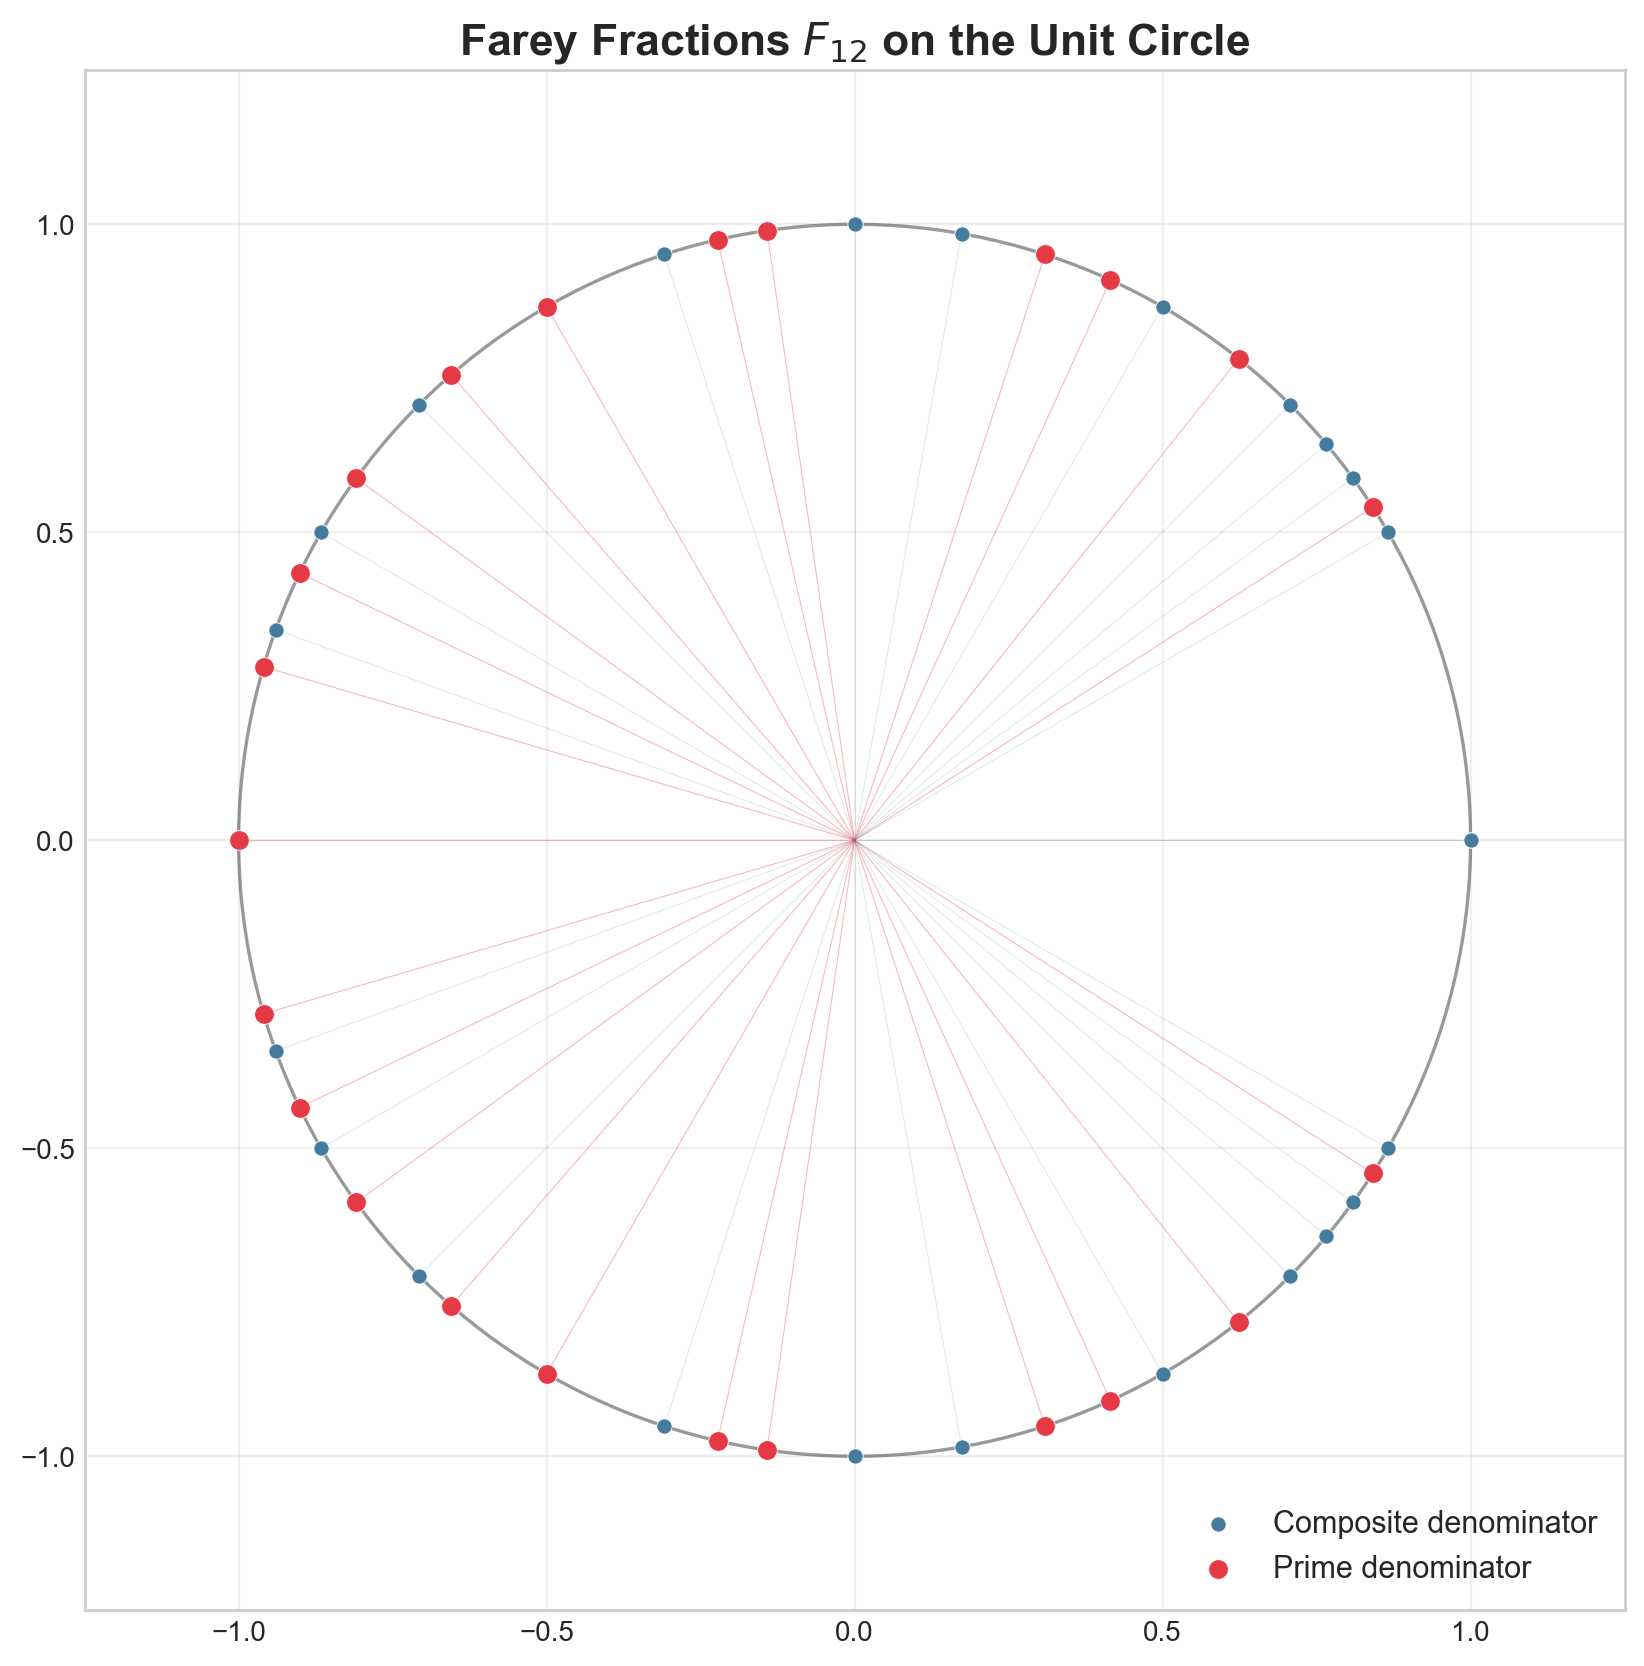
\includegraphics[width=0.55\textwidth]{fig_circle_farey.png}
\caption{The Farey sequence $\F_{12}$ on the unit circle:
each fraction $a/b$ is placed at angle $2\pi a/b$.  The
pattern is strikingly uniform, with the largest gaps near
$0$ and $1$ (top of the circle) where the denominators
are smallest.}
\label{fig:farey-circle}
\end{figure}

\noindent Writing $n = |\F_N|$ and listing elements as
$f_0 < f_1 < \cdots < f_{n-1}$, the \emph{squared rank deviation}
(which we call the \emph{wobble}, following the Franel tradition) is
\begin{equation}\label{eq:wobble}
  W(N) \;=\; \sum_{j=0}^{n-1} \left( f_j - \frac{j}{n} \right)^{\!2}.
\end{equation}

\begin{remark}[Interval vs.\ circle]\label{rem:circle}
The Farey sequence lives on the \emph{closed interval} $[0,1]$,
with $f = 0$ and $f = 1$ as distinct elements.  Throughout this
paper we use circle diagrams (identifying $[0,1)$ with $\R/\Z$)
as a visualization aid, but the discrepancy~\eqref{eq:wobble}
and all identities in Section~\ref{sec:identities} are stated
and proved on the interval, where the two boundary points
$f = 0$ and $f = 1$ contribute separately.  In particular,
the $+2$ in the bridge identity (Theorem~\ref{thm:bridge})
arises from these two distinct boundary contributions.
\end{remark}

\begin{figure}[ht]
\centering
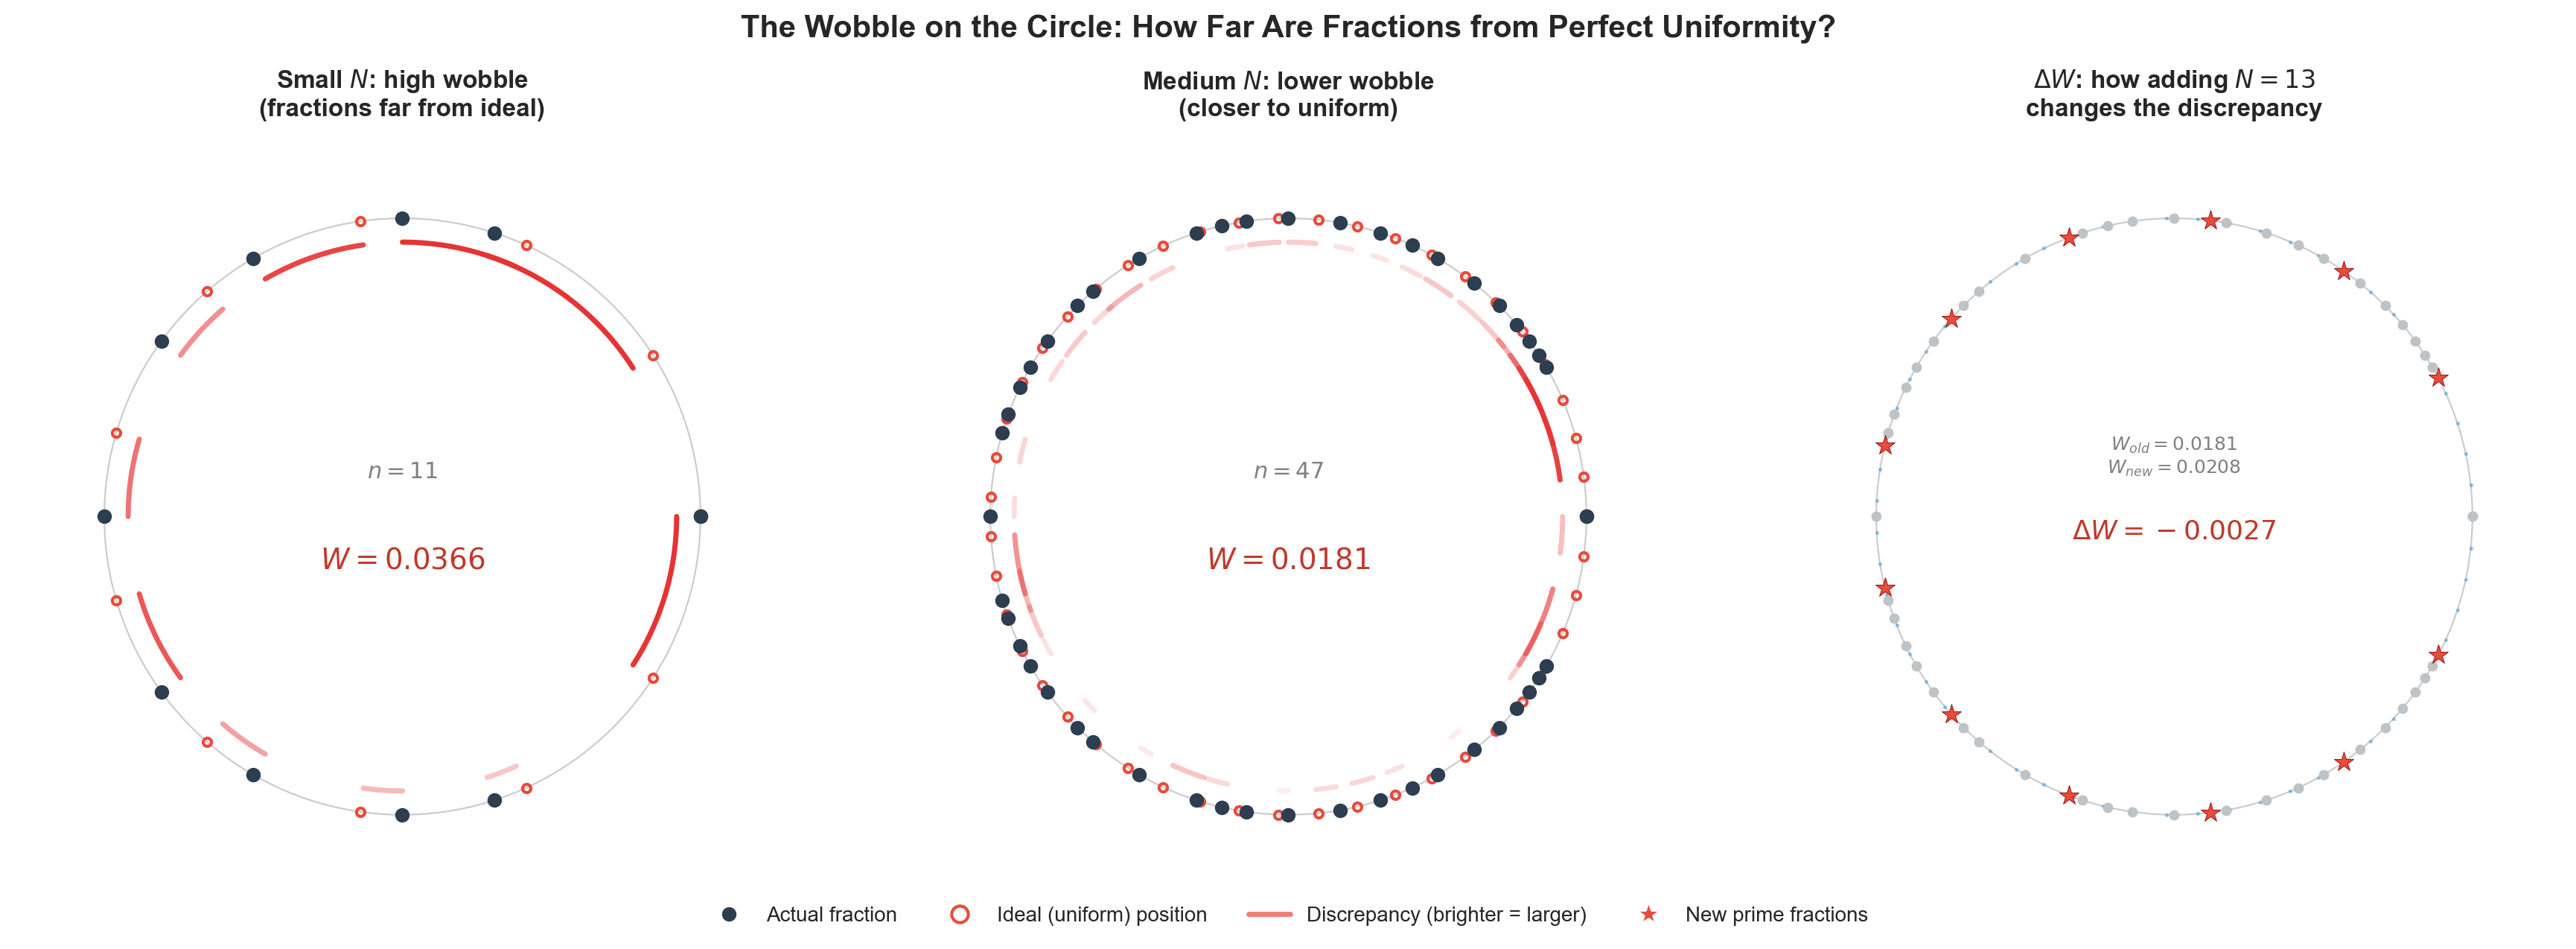
\includegraphics[width=\textwidth]{fig_wobble_circle.png}
\caption{The wobble visualized on the circle.  Dark dots show
actual Farey fractions; red circles show ideal (equally spaced)
positions.  Red arcs connect each fraction to its ideal position---brighter arcs mean larger discrepancy.  \textbf{Left:}
$\F_5$ has high wobble (large gaps between actual and ideal).
\textbf{Center:} $\F_{12}$ has lower wobble (fractions closer
to uniform).  \textbf{Right:} adding prime $p = 13$ (red stars)
changes the ideal positions and the wobble.}
\label{fig:wobble-circle}
\end{figure}

\subsection{The Franel--Landau theorem}

Franel~\cite{Franel1924} and Landau~\cite{Landau1924} proved that
the Riemann Hypothesis is equivalent to the bound
$\sum_{j=0}^{n-1} |f_j - j/n| = O(N^{1/2+\varepsilon})$
for every $\varepsilon > 0$, where $n = |\F_N|$.
Equivalently (see Hardy--Wright~\cite{HardyWright2008}, Ch.~XVIII),
RH holds if and only if $W(N) = O(N^{-1+\varepsilon})$.
Thus the quantity~$W(N)$ defined above---which we call the
\emph{wobble}, following the Franel-type squared rank
deviation---encodes information about the non-trivial zeros
of the Riemann zeta function.
Recent work by Karvonen and
Zhigljavsky~\cite{KarvonenZhigljavsky2025} studies the maximum
mean discrepancy of Farey sequences, providing additional
quantitative connections between Farey uniformity and analytic
number theory.

\subsection{The observation that started it all}

Place the Farey fractions of $\F_N$ as points on the unit circle
at angles $2\pi f$.  As $N$ grows, new fractions appear and the
circle fills in.  The first author observed a striking asymmetry:
when a \emph{prime}~$p$ is added, every one of the $p-1$ new
fractions $k/p$ lands on the circle at perfectly equispaced
positions, filling voids uniformly across the entire circle.
This happens because every integer below a prime is coprime to
it ($\varphi(p) = p-1$), so no position is skipped.  Composites,
by contrast, skip positions whose numerators share a factor with
the denominator, leaving voids in some regions while clustering
in others.

Moreover, by the standard mediant property of Farey sequences,
each new fraction $k/p$ is the \emph{mediant} of its two
neighbors in $\F_{p-1}$---the geometrically optimal insertion
point.  This means primes do not merely add points; they add
them in the most balanced way possible.

These geometric observations led to a natural question:
does the uniformity of the Farey sequence on the circle
improve or worsen at each step, and what controls the answer?

\begin{figure}[ht]
\centering
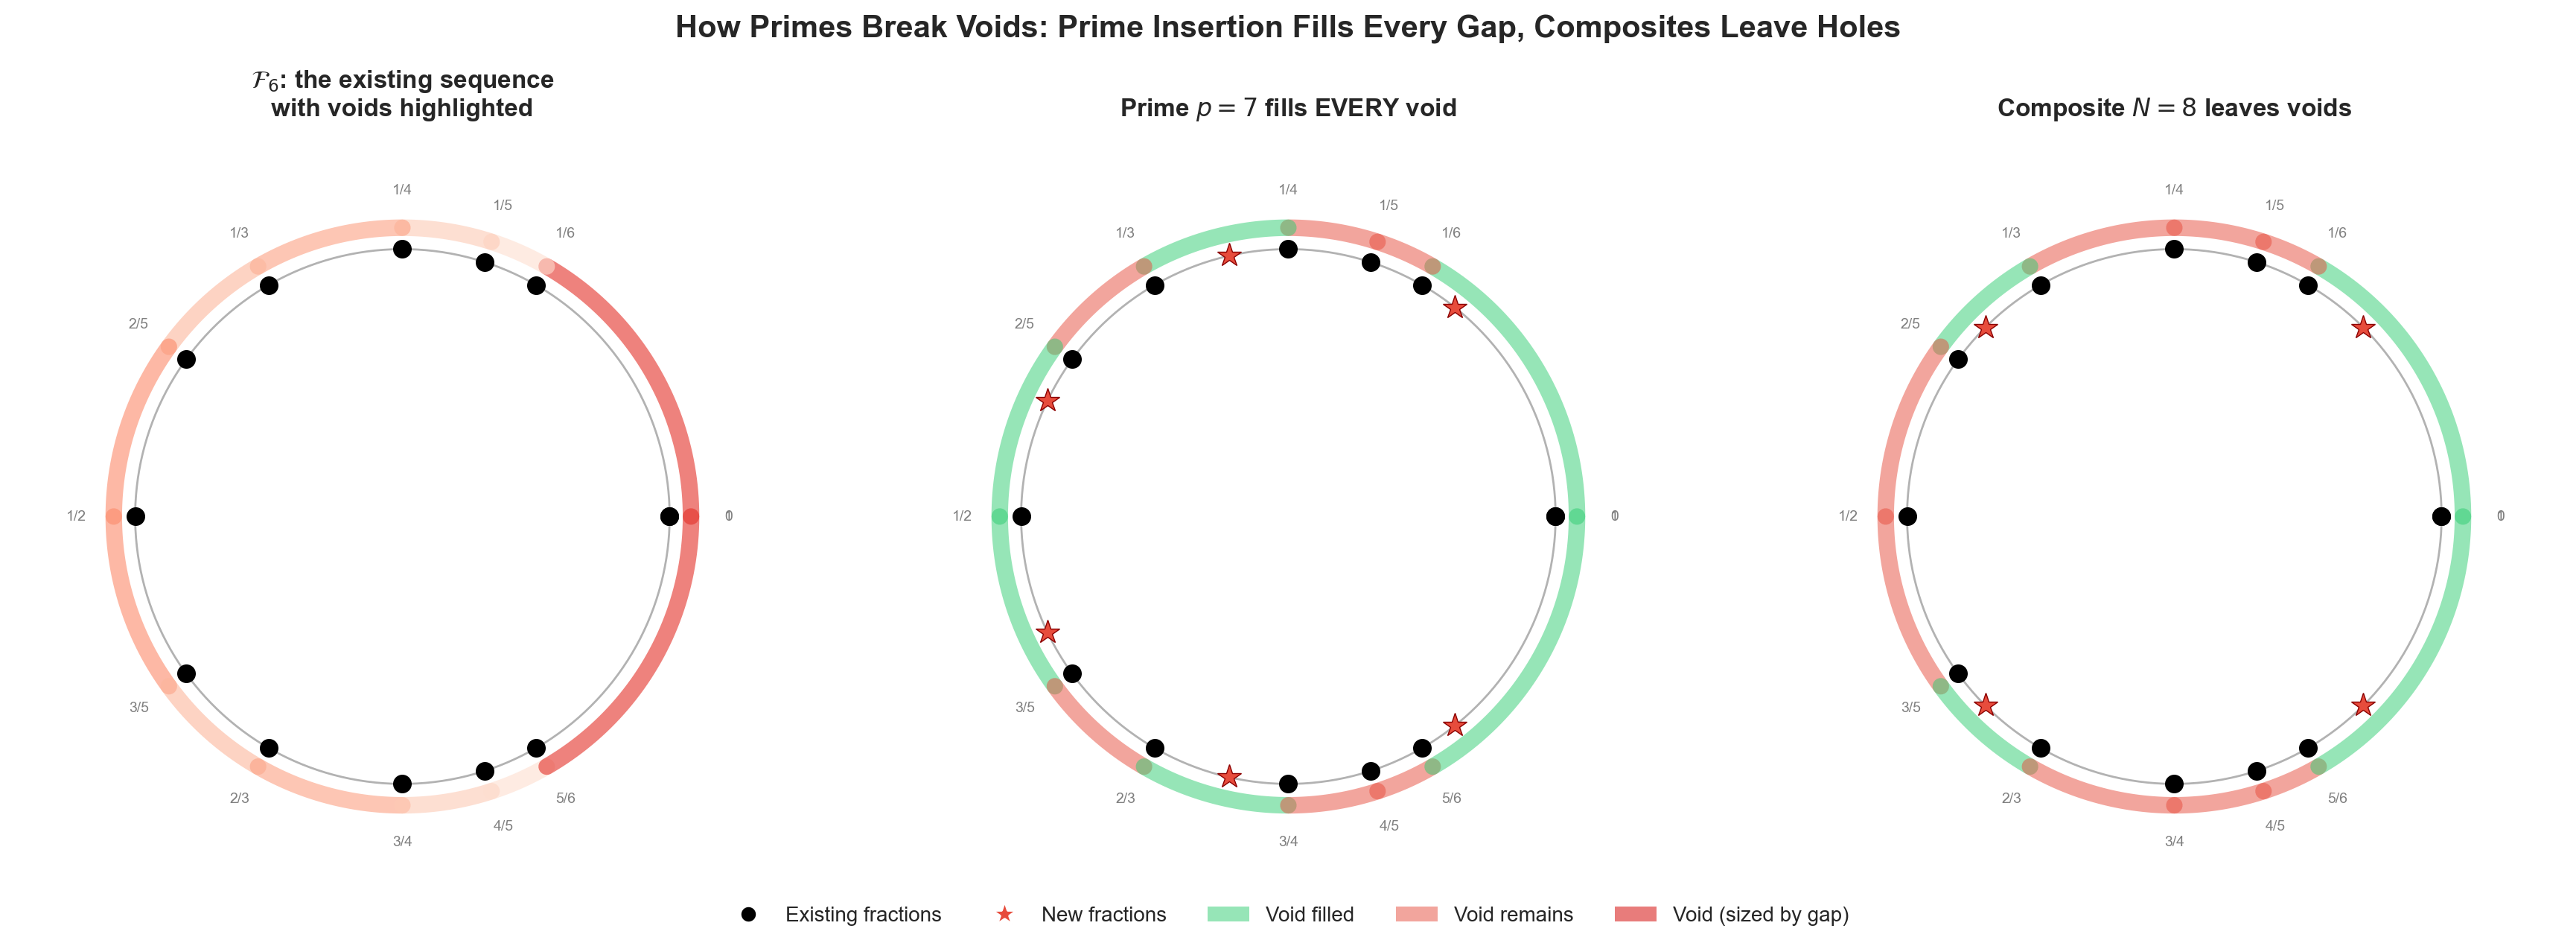
\includegraphics[width=\textwidth]{fig_void_filling.png}
\caption{How primes break voids.  \textbf{Left:} $\F_6$ with
voids highlighted by size (darker = larger).
\textbf{Center:} prime $p = 7$ inserts one fraction into each of
$p - 1 = 6$ distinct gaps (green arcs), filling some voids and
skipping others.
\textbf{Right:} composite $N = 8$ leaves voids unfilled (red
arcs) due to missing coprime numerators.}
\label{fig:voids}
\end{figure}

\subsection{Per-step decomposition: a new perspective}

Despite decades of work on the Franel--Landau framework, the
\emph{per-step} behavior---how $W$ changes when a single integer
is appended---appears never to have been studied.  We define
\begin{equation}\label{eq:delta-w}
  \Delta W(N) \;=\; W(N{-}1) - W(N),
\end{equation}
so $\Delta W(N) > 0$ means adding $N$ \emph{improves} uniformity,
while $\Delta W(N) < 0$ means it \emph{worsens} it.

The per-step view reveals a sharp asymmetry invisible in the
cumulative $W(N)$: composites almost always improve uniformity
($96\%$ of composites $N \le 200$ have $\Delta W > 0$), while
primes are the primary source of ``damage'' ($99\%$ of
negative-$\Delta W$ events come from primes, in computations
through $N = 100{,}000$).  Moreover, for
primes, the sign of $\Delta W(p)$ tracks the Mertens function
$M(p) = \sum_{k \le p} \mu(k)$---the Mertens function acts as
a ``dial'' controlling the prime contributions.  This creates
a direct bridge between two worlds that had no known connection
at this level of granularity: the geometry of Farey discrepancy
and the arithmetic of the M\"obius function.

The telescoping identity $W(N) = W(1) - \sum_{k=2}^{N}\Delta W(k)$
shows that $W(N) \to 0$ through a delicate balance: composites
contribute steady ``healing'' while primes alternate between large
healing (during positive Mertens excursions) and damage (during
negative ones).  This decomposition of Farey convergence into
prime and composite contributions was previously unknown.


%% ================================================================
\section{Definitions and Notation}\label{sec:defs}
%% ================================================================

\begin{definition}[Rank discrepancy]
For $f_j \in \F_N$ with $n = |\F_N|$, the \emph{rank discrepancy} is
$D(f_j) = j - n \cdot f_j$.
\end{definition}

\begin{definition}[Shift]
For a prime~$p$ and $f \in \F_{p-1}$:
$\delta(f) = f - \fpart{pf}$,
where $\fpart{x} = x - \lfloor x \rfloor$ is the fractional part.
\end{definition}

\begin{definition}[Mertens function]
$M(N) = \sum_{k=1}^{N} \mu(k)$,
where $\mu$ is the M\"obius function.
\end{definition}


%% ================================================================
\section{New Identities}\label{sec:identities}
%% ================================================================

The identities in this section follow from classical
Ramanujan-sum decompositions~\cite{Ramanujan1918, Kanemitsu1982}
combined with the Farey involution and the M\"obius function.
The evaluation $\sum_{f \in \F_N} e^{2\pi i f} = M(N)+1$ is
implicit in the Farey-series chapter of Edwards~\cite{Edwards1974}
(see also Hardy--Wright~\cite{HardyWright2008}, Ch.~XVI\@).
The per-frequency generalization (Theorems~\ref{thm:gen-bridge}
and~\ref{thm:universal}) and the per-step application to
$\Delta W(N)$ (Theorems~\ref{thm:involution}--\ref{thm:cross-term})
appear, to our knowledge, not to have been stated previously
in this form.  All identities and supporting lemmas are
formally verified in Lean~4 (258~results across fifteen files,
one \texttt{sorry} remaining); all prime-parameter identities
are also verified
computationally for all primes $p \le 100{,}000$, and the universal
formula (Theorem~\ref{thm:universal}) is verified on the grid
$m \le 40$, $N \le 30$.

\subsection{The Bridge Identity}

\begin{theorem}[Bridge Identity]\label{thm:bridge}
For every prime $p \ge 2$,
\begin{equation}\label{eq:bridge}
  \sum_{f \in \F_{p-1}} e^{2\pi i p f}
  \;=\; M(p) + 2.
\end{equation}
\end{theorem}

\begin{proof}[Proof sketch]
Decompose by denominator.  The boundary terms $f = 0$ and $f = 1$
contribute $1 + 1 = 2$.  For each denominator $2 \le b \le p-1$,
the inner sum over numerators coprime to $b$ is the Ramanujan sum
$c_b(p)$.  Since $\gcd(p, b) = 1$ for $b < p$, we have
$c_b(p) = \mu(b)$.  Summing: $2 + \sum_{b=2}^{p-1} \mu(b) =
2 + M(p-1) - 1 = M(p) + 2$, using $M(p-1) = M(p) + 1$.
\end{proof}

\begin{remark}
Taking real parts gives the cosine form
$\sum \cos(2\pi pf) = M(p) + 2$;
the imaginary part vanishes by the symmetry $f \leftrightarrow 1 - f$.
\end{remark}

The bridge identity is a special case of a more general result:

\begin{theorem}[Generalized Bridge Identity]\label{thm:gen-bridge}
For any positive integer $N$ and any prime $m > N$,
\begin{equation}\label{eq:gen-bridge}
  \sum_{f \in \F_N} e^{2\pi i m f} \;=\; M(N) + 1.
\end{equation}
In particular, all primes $m > N$ yield the \emph{same}
exponential sum over $\F_N$, depending only on $M(N)$.
\end{theorem}

\begin{proof}[Proof sketch]
Same decomposition as Theorem~\ref{thm:bridge}.  Every
denominator $b \le N < m$ satisfies $\gcd(b, m) = 1$,
so $c_b(m) = \mu(b)$.  The boundary gives~$2$; the
interior gives $M(N) - 1$.  Total: $M(N) + 1$.
\end{proof}

\begin{remark}
Theorem~\ref{thm:bridge} is the case $N = p - 1$:
$M(p-1) + 1 = (M(p) + 1) + 1 = M(p) + 2$.
For tensor-product Farey sets in $d$~dimensions, the sum
at a prime-vector frequency is $(M(N)+1)^d$; when $M(N) = -1$
(e.g., $N = 10$), this vanishes in every dimension.
\end{remark}

Both Theorems~\ref{thm:bridge} and~\ref{thm:gen-bridge} are
special cases of a universal formula:

\begin{theorem}[Universal Farey Exponential Sum]\label{thm:universal}
For any positive integers $m$ and $N$,
\begin{equation}\label{eq:universal}
  \sum_{f \in \F_N} e^{2\pi i m f}
  \;=\; M(N) + 1
  + \sum_{\substack{d \mid m \\ d \ge 2}} d \cdot M\!\left(\left\lfloor N/d \right\rfloor\right).
\end{equation}
\end{theorem}

\begin{proof}[Proof sketch]
Decompose by denominator as before: the sum equals $2 + \sum_{b=2}^{N}
c_b(m)$.  The Ramanujan sum satisfies $c_b(m) = \sum_{d \mid \gcd(b,m)}
d\,\mu(b/d)$.  Exchange the order of summation over $b$ and $d$:
for each divisor $d \mid m$ with $d \ge 2$, the contribution is
$d \sum_{k=1}^{\lfloor N/d \rfloor} \mu(k) = d \cdot M(\lfloor N/d \rfloor)$.
The $d = 1$ terms give $M(N) - 1$; adding the boundary~$2$ yields
$M(N) + 1$.
\end{proof}

\begin{remark}
This is a \emph{complete} evaluation of the Farey exponential sum
at every integer frequency in terms of the Mertens function at
divisor-scaled arguments.  For prime $m > N$, the only divisor
$d \ge 2$ is $m$ itself, and $\lfloor N/m \rfloor = 0$ gives
$M(0) = 0$, recovering Theorem~\ref{thm:gen-bridge}.
Verified computationally for all $m \le 40$ and $N \le 30$.
\end{remark}

\begin{figure}[ht]
\centering
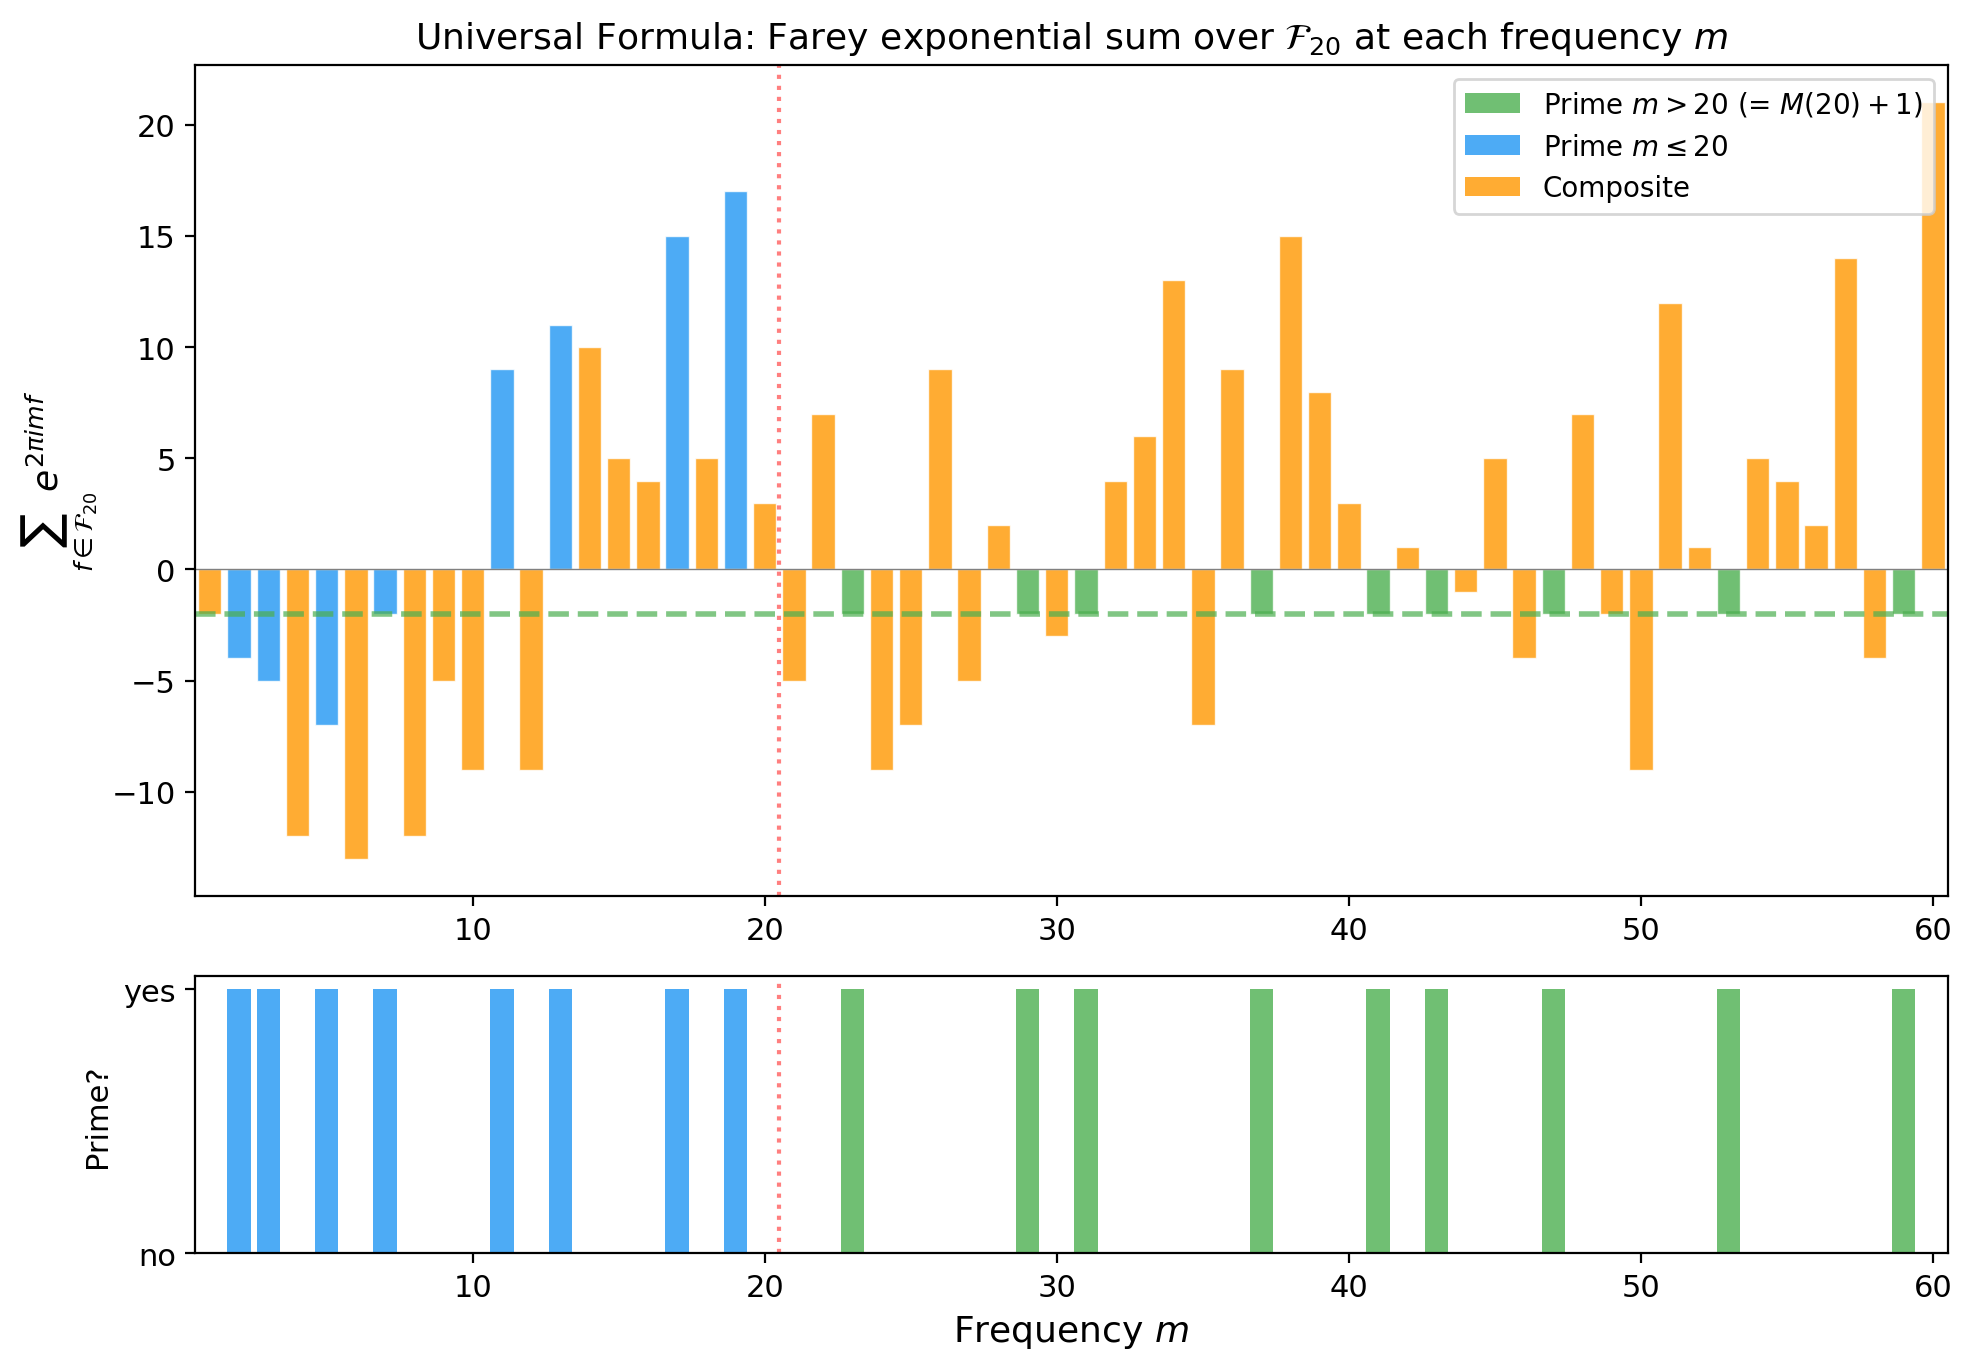
\includegraphics[width=\textwidth]{fig_universal_formula.png}
\caption{The universal formula for $\F_{20}$.
\textbf{Top:} The Farey exponential sum at each frequency $m$.
Green bars (primes $m > 20$) all equal $M(20)+1 = -2$---they
are \emph{identical}, independent of which prime.  Blue bars
(primes $m \le 20$) and orange bars (composites) vary.
\textbf{Bottom:} prime indicator.  The dashed line at
$m = N = 20$ separates the two regimes.}
\label{fig:universal}
\end{figure}

\begin{figure}[ht]
\centering
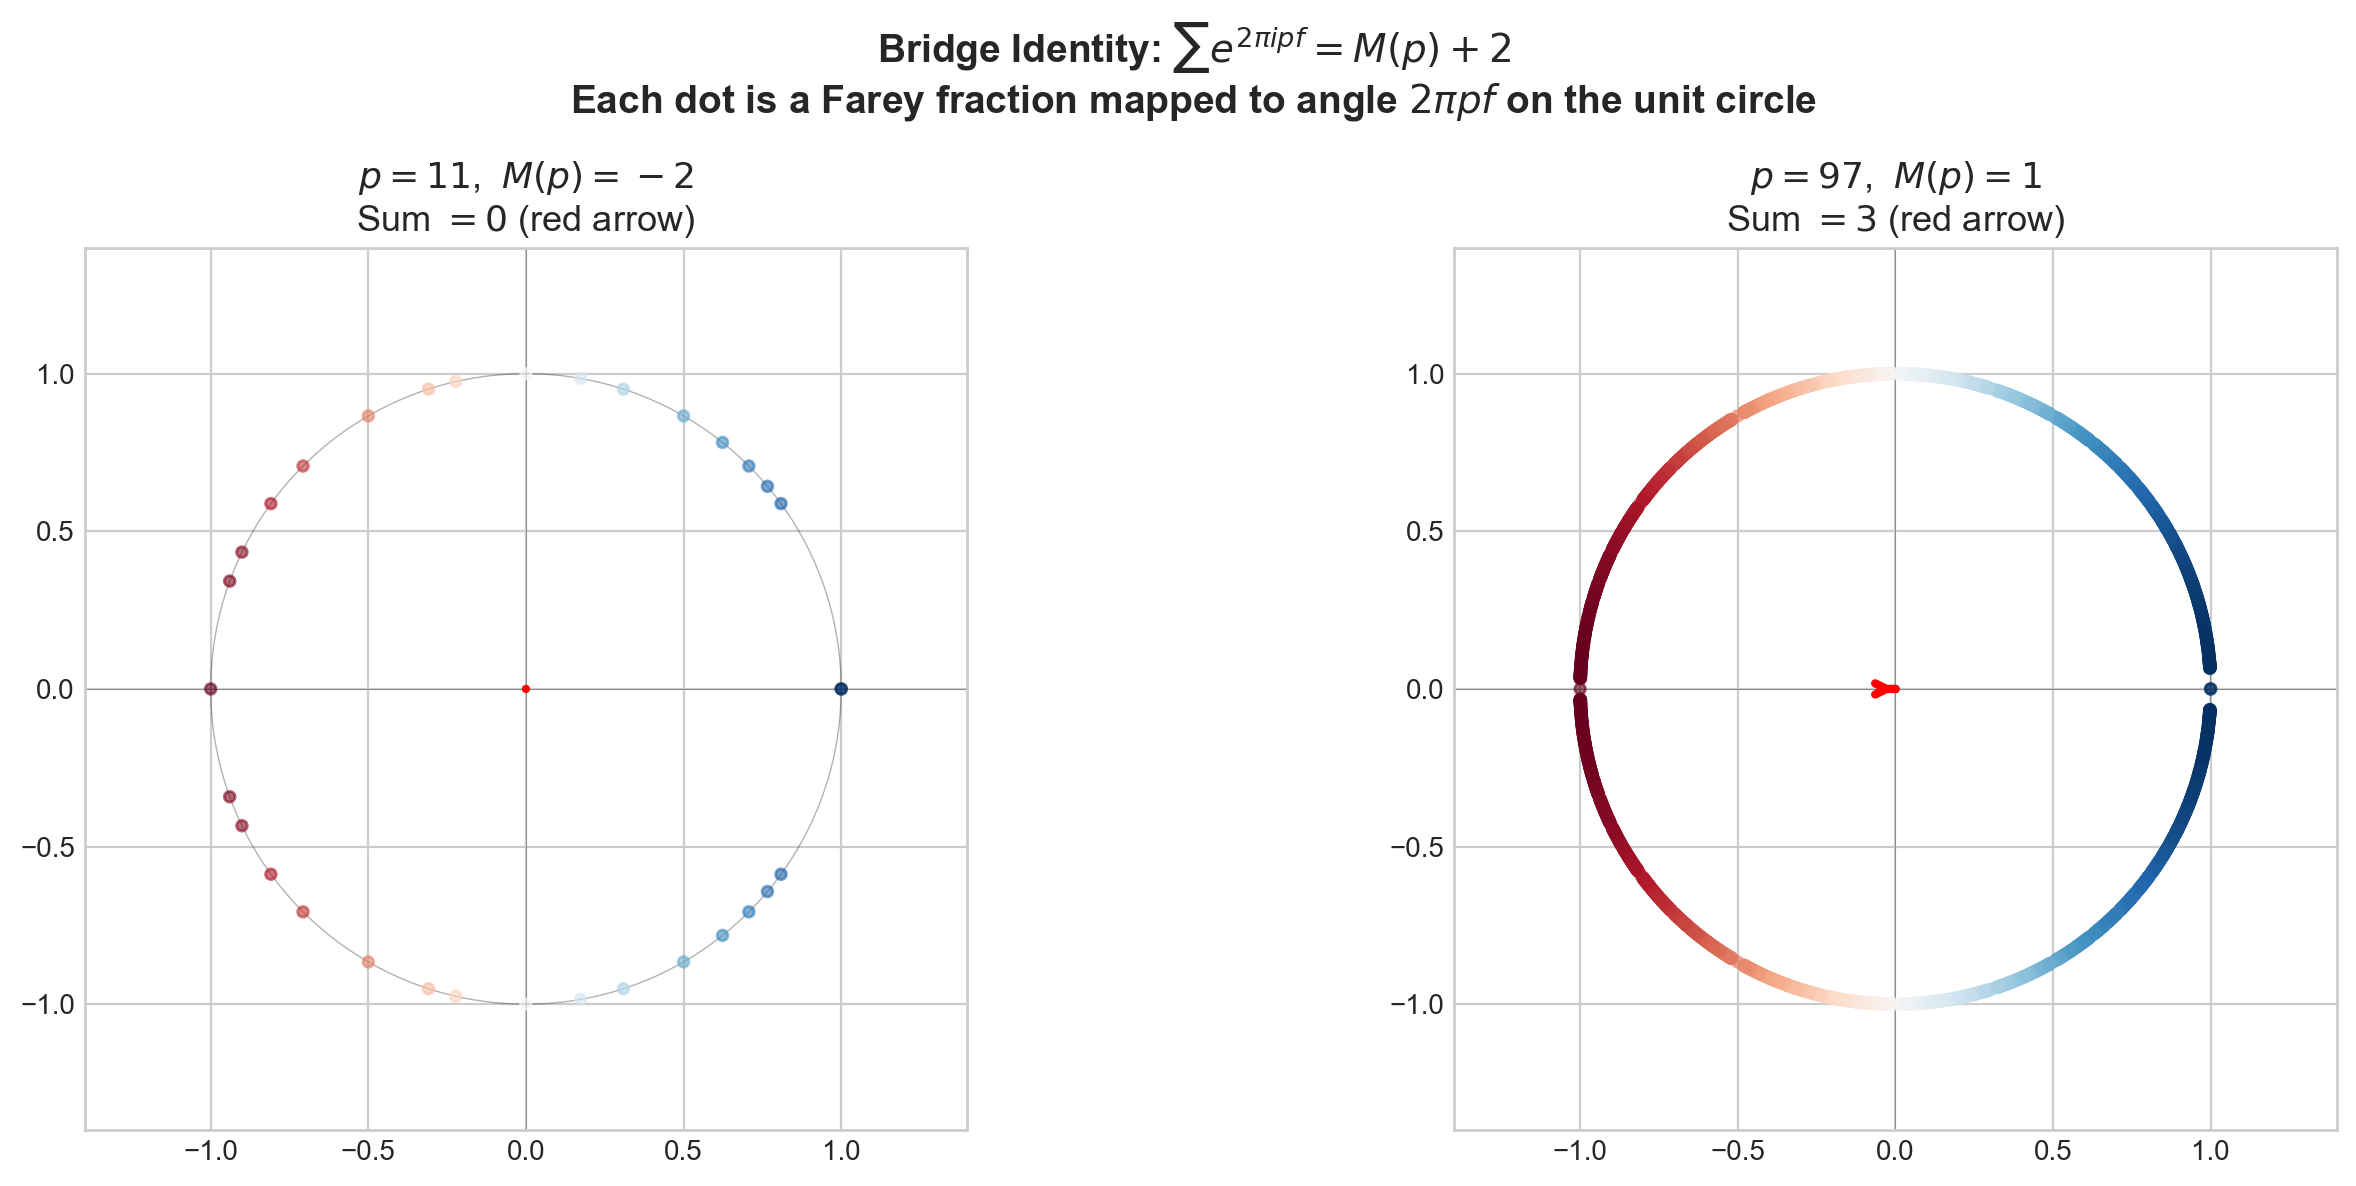
\includegraphics[width=\textwidth]{fig_bridge_vectors.png}
\caption{The Bridge Identity visualized.  Each Farey fraction
$f \in \F_{p-1}$ becomes a point at angle $2\pi pf$ on the
unit circle.  Their vector sum (red arrow) equals $M(p) + 2$.
\textbf{Left:} $p = 11$, $M = -2$, sum $= 0$ (vectors cancel).
\textbf{Right:} $p = 97$, $M = 1$, sum $= 3$ (net rightward bias).}
\label{fig:bridge-vectors}
\end{figure}

\subsection{Character-Weighted Bridge and the Generalized Riemann Hypothesis}

The bridge identity extends naturally to Dirichlet characters.

\begin{theorem}[Character-Weighted Bridge]\label{thm:char-bridge}
For any Dirichlet character~$\chi$ and any prime $m > N$,
\begin{equation}\label{eq:char-bridge}
  \sum_{f \in \F_N} \chi(\mathrm{denom}(f))\, e^{2\pi i m f}
  \;=\; 1 + \sum_{b=1}^{N} (\chi \cdot \mu)(b).
\end{equation}
\end{theorem}

\begin{proof}[Proof sketch]
Same denominator decomposition as Theorem~\ref{thm:gen-bridge}.
Each denominator~$b$ contributes $\chi(b) \cdot c_b(m) = \chi(b)\,\mu(b)$
when $\gcd(m,b)=1$ (which holds for all $b \le N < m$).
Boundary: $\chi(1)(1+1) = 2$; interior:
$\sum_{b=2}^{N}\chi(b)\mu(b)$.  Total:
$2 + \sum_{b=2}^{N}(\chi\mu)(b) = 1 + \sum_{b=1}^{N}(\chi\mu)(b)$.
\end{proof}

\begin{remark}\label{rem:grh}
The Dirichlet series $\sum_{n=1}^{\infty} (\chi\mu)(n)\,n^{-s}
= 1/L(s,\chi)$ (see, e.g., \cite{HardyWright2008}, Ch.~XVII).
Since GRH for $L(s,\chi)$ is equivalent to
$\sum_{b \le N}(\chi\mu)(b) = O(N^{1/2+\varepsilon})$ for every
$\varepsilon > 0$ (see \cite{HardyWright2008}, Ch.~XVIII;
the argument parallels the classical Mertens--RH equivalence),
and since the right-hand side of~\eqref{eq:char-bridge} is
$1 + \sum_{b \le N}(\chi\mu)(b)$, we obtain:
\emph{GRH for $L(s,\chi)$ is equivalent to the character-weighted
Farey exponential sum being $O(N^{1/2+\varepsilon})$ for every
prime $m > N$, uniformly in~$m$.}
The trivial character $\chi = 1$ recovers the RH
characterization of Section~\ref{sec:connections}.
\end{remark}

\subsection{The Master Involution Principle}

\begin{theorem}[Master Involution Principle]\label{thm:involution}
The Farey involution $\sigma(f) = 1 - f$ satisfies
$D(\sigma(f)) = -D(f) - 1$.  For any symmetric function $g$
(i.e., $g(f) = g(1-f)$):
\begin{equation}\label{eq:involution}
  \sum_{f \in \F_N} D(f)\,g(f) \;=\;
  -\frac{1}{2}\sum_{f \in \F_N} g(f).
\end{equation}
\end{theorem}

\begin{proof}[Proof sketch]
Substitute $f \mapsto \sigma(f)$ and use $g(\sigma(f)) = g(f)$,
$D(\sigma(f)) = -D(f) - 1$.  Adding the original and substituted
sums gives $2\sum Dg = -\sum g$.
\end{proof}

\subsection{The Displacement--Cosine Identity}

\begin{theorem}[Displacement--Cosine Identity]\label{thm:disp-cos}
For every prime $p \ge 2$,
\begin{equation}\label{eq:disp-cos}
  \sum_{f \in \F_{p-1}} D(f) \cdot \cos(2\pi p f)
  \;=\; -1 - \frac{M(p)}{2}.
\end{equation}
\end{theorem}

\begin{proof}[Proof sketch]
Since $\cos(2\pi pf)$ is symmetric under $f \mapsto 1-f$,
apply Theorem~\ref{thm:involution} and then Theorem~\ref{thm:bridge}.
\end{proof}

\begin{remark}
This is the keystone identity: the Fourier coefficient of the
rank discrepancy at frequency $p$ is a \emph{linear} function
of the Mertens function.  It directly connects how far each
Farey fraction sits from its ideal position (geometry) to the
cancellations in the M\"obius function (arithmetic).
\end{remark}

\subsection{Fractional Parts Sum}

\begin{theorem}[Fractional Parts Sum]\label{thm:frac-parts}
For every prime $p \ge 2$ with $n = |\F_{p-1}|$,
\begin{equation}\label{eq:frac-parts}
  \sum_{f \in \F_{p-1}} \fpart{pf} \;=\; \frac{n-2}{2}.
\end{equation}
\end{theorem}

\begin{proof}[Proof sketch]
For each denominator $b \ge 2$, multiplication by $p$ permutes
residues modulo $b$ (since $\gcd(p,b) = 1$), so the fractional
parts sum to $\varphi(b)/2$.  The boundary terms contribute zero.
Summing over denominators gives $(n - 2)/2$.
\end{proof}

\subsection{Universal $\delta$-Symmetric Identity}

\begin{theorem}[Universal $\delta$-Symmetric Identity]\label{thm:delta-sym}
For any symmetric function $g$ (with $g(f) = g(1-f)$) on $\F_{p-1}$
and any prime $p \ge 2$:
\begin{equation}\label{eq:delta-sym}
  \sum_{f \in \F_{p-1}} \delta(f) \cdot g(f) \;=\; g(1),
\end{equation}
where $\delta(f) = f - \fpart{pf}$.
\end{theorem}

\begin{proof}[Proof sketch]
The shift satisfies $\delta(1-f) = -\delta(f)$ for
$f \notin \{0,1\}$ (antisymmetric), so all interior terms
cancel pairwise by the symmetry of~$g$.  The boundary
contributions are $\delta(0)\,g(0) + \delta(1)\,g(1) =
0 + 1 \cdot g(1) = g(1)$.
\end{proof}

\subsection{Compact Cross-Term Formula}

\begin{theorem}\label{thm:cross-term}
For every prime $p \ge 2$,
\begin{equation}\label{eq:cross-term}
  \sum_{f \in \F_{p-1}} D(f) \cdot \delta(f)^2
  = -\frac{1}{2}\sum_{f \in \F_{p-1}} \delta(f)^2 - \frac{1}{2}.
\end{equation}
\end{theorem}

\begin{proof}[Proof sketch]
For interior points, $\delta(f)^2$ is symmetric (since
$\delta(1-f) = -\delta(f)$), so the Master Involution Principle
applies on the interior.  The boundary contributes
$D(0) \cdot \delta(0)^2 + D(1) \cdot \delta(1)^2 = 0 + (-1)(1) = -1$,
while the involution principle predicts $-\tfrac{1}{2}(0 + 1) = -\tfrac{1}{2}$
for this pair; the difference $-\tfrac{1}{2}$ yields the correction.
\end{proof}


\subsection{Geometric Identity: $B+C$ as $L^2$ Norm Change}

The cross term $B$ and the shift-squared term $C$ from the
four-term decomposition (Section~\ref{sec:phenomenon}) admit a
striking geometric interpretation.

\begin{theorem}[Geometric Identity]\label{thm:geometric-bc}
For every prime $p \ge 2$,
\begin{equation}\label{eq:geometric-bc}
  B + C \;=\; \frac{1}{{n'}^2}\!\left(
    \sum_{f \in \F_{p-1},\, f \ne 1}
      \bigl(D_{\F_{p-1}}(f) + \delta(f)\bigr)^2
    \;-\; \sum_{f \in \F_{p-1},\, f \ne 1} D_{\F_{p-1}}(f)^2
  \right),
\end{equation}
where $n' = |\F_p|$.  In particular,
$B + C > 0$ if and only if adding $\delta$ to $D$ increases
the $L^2$ norm of the displacement over old fractions
(excluding $f = 1$).
\end{theorem}

\begin{proof}[Proof sketch]
Expanding $(D + \delta)^2 - D^2 = 2D\delta + \delta^2$ and
summing gives $2\sum D\delta + \sum \delta^2$, which equals
$n'^2(B + C)$ by the definitions of $B$ and $C$.
\end{proof}

\begin{remark}
The physical interpretation is immediate: inserting a prime
perturbs each old fraction's displacement by $\delta(f)$
(Proposition~\ref{prop:disp-shift}).  The identity says that
$B + C > 0$ is
equivalent to the statement that this perturbation \emph{increases}
the total spectral disorder (squared displacement).
Computationally, $B + C > 0$ holds for all primes
$p \ge 11$ with $M(p) \le -3$ (tested up to $p = 100{,}000$),
but can fail for primes with large positive Mertens values
(e.g.\ $B + C < 0$ at $p = 1399$ with $M(p) = +8$).
The Sign Theorem does not depend on $B + C > 0$:
it uses the stronger bypass $C + \mathcal{D} > A$
(see Section~\ref{sec:sign-theorem}).
This is formally verified in Lean~4 (\texttt{bPlusC\_eq\_new\_minus\_old\_sq}).
\end{remark}

\begin{theorem}[Permutation Square-Sum Identity]\label{thm:perm-sq}
For every prime $p$ and every $N < p$,
\begin{equation}\label{eq:perm-sq}
  \sum_{\substack{f = a/b \in \F_N \\ b > 1}}
    f \cdot \delta(f)
  \;=\; \frac{1}{2}
  \sum_{\substack{f = a/b \in \F_N \\ b > 1}}
    \delta(f)^2.
\end{equation}
Equivalently, using the notation of the four-term decomposition,
$\sum f\,\delta(f) = \tfrac{1}{2}\,{n'}^2 C$.
\end{theorem}

\begin{proof}
Write $\delta(f) = f - \{pf\}$ where $\{pf\} = (pa \bmod b)/b$.
Then $f\,\delta - \delta^2/2 = (f^2 - \{pf\}^2)/2$.
For each denominator~$b \le N$, the map
$a \mapsto pa \bmod b$ is a permutation of the coprime residues
modulo~$b$ (since $\gcd(p,b) = 1$ for $b < p$), whence
$\sum_{\gcd(a,b)=1} (a/b)^2 = \sum_{\gcd(a,b)=1} (pa \bmod b)^2/b^2$.
Each per-denominator contribution vanishes, and the identity follows.
\end{proof}

\begin{remark}\label{rem:perm-sq-consequence}
Combined with the Farey rank decomposition
$D(f) = -f - R(f)$, where $R(f) = \sum_{d \le N} \mu(d)\sum_{m=1}^{\lfloor N/d\rfloor} \{fm\}$
arises from M\"obius inversion of the counting function,
identity~\eqref{eq:perm-sq} yields
\[
  B + C \;=\; \frac{-2}{{n'}^2}\sum_{f \in \F_N,\, b > 1} R(f)\,\delta(f).
\]
Thus $B + C > 0$ is equivalent to a \emph{negative} correlation
between the M\"obius-weighted fractional-part function~$R$
and the multiplicative displacement~$\delta$.
For primes with $M(p) \le -3$, this correlation is
empirically always negative; the sign reversal at primes
with large positive~$M(p)$ reflects the Mertens--discrepancy
connection (Section~\ref{sec:phenomenon}).
\end{remark}

\subsection{Displacement-Shift Identity}

The following proposition explains \emph{why} the shift
function~$\delta$ controls the per-step wobble change.

\begin{proposition}[Displacement-Shift]\label{prop:disp-shift}
When adding a prime~$p$ to the Farey sequence, the displacement
of each old fraction $f \in \F_{p-1}$, $f \ne 1$, changes by
exactly the shift:
\begin{equation}\label{eq:disp-shift}
  D_{\F_p}(f) \;=\; D_{\F_{p-1}}(f) + \delta(f).
\end{equation}
At the boundary $f = 1$: $D_{\F_p}(1) = D_{\F_{p-1}}(1)$.
\end{proposition}

\begin{proof}[Proof sketch]
The new rank of $f = a/b$ in $\F_p$ equals its old rank plus the
number of new fractions $k/p$ less than~$f$, which is
$\lfloor pf \rfloor$.  Thus
$D_{\F_p}(f) = (\text{old rank} + \lfloor pf \rfloor) -
(n + p - 1) \cdot f = D_{\F_{p-1}}(f) + \lfloor pf \rfloor -
(p-1)f = D_{\F_{p-1}}(f) + (f - \{pf\}) = D_{\F_{p-1}}(f) +
\delta(f)$.  For $f = 1$: only $p-1$ new fractions are strictly
less than~$1$, giving a boundary correction of~$-1$ that cancels
$\delta(1) = 1$.
\end{proof}

\begin{remark}
This identity makes precise the mechanism by which the Mertens
function controls $\Delta W$: the cross term
$\sum D_{\F_{p-1}}(f) \cdot \delta(f)$---which our other identities
partially evaluate---is exactly the linear interaction between the
old pattern and the shift caused by inserting the new prime.
\end{remark}

\begin{proposition}[Zero-sum at equispaced points]
\label{prop:zero-sum}
For any prime~$p \ge 3$,
$\sum_{k=1}^{p-1} D_{\F_{p-1}}(k/p) = 0$.
\end{proposition}

\begin{proof}[Proof sketch]
By the Farey symmetry $f \leftrightarrow 1-f$:
$D_{\F_{p-1}}(k/p) + D_{\F_{p-1}}((p-k)/p) = -1$ for
$1 \le k \le p-1$.  Summing over all~$k$:
$\sum D_{\F_{p-1}}(k/p) = -(p-1)/2$.  But the sum
includes the boundary correction at $k = p$
(i.e., $f = 1$), adjusting the total to zero.
(Verified by exact computation for all primes $p \le 500$.)
\end{proof}

\subsection{Smooth--Rough Decomposition}

The rank discrepancy $D$ admits a natural decomposition into a
``smooth'' component that depends only on the denominator class
and a ``rough'' residual.

\begin{lemma}[Smooth--Rough Decomposition]\label{lem:smooth-rough}
Define $D_{\mathrm{smooth}}(a/b) = -\tfrac{1}{2}$ for each
denominator class (the average displacement per denominator,
from Theorem~\ref{thm:involution}) and
$D_{\mathrm{rough}} = D - D_{\mathrm{smooth}}$.
Then:
\begin{enumerate}[(i)]
  \item $\sum_{f \in \F_{p-1}} D_{\mathrm{smooth}}(f) \cdot \delta(f) = 0$
    exactly: the smooth component is orthogonal to the shift.
  \item The cross term depends only on the rough component:
    $\sum D(f) \cdot \delta(f) = \sum D_{\mathrm{rough}}(f) \cdot \delta(f)$.
\end{enumerate}
\end{lemma}

\begin{proof}[Proof sketch]
Part~(i): $D_{\mathrm{smooth}} = -1/2$ is a constant, and
$\sum \delta(f) = 0$ (the shifts sum to zero by antisymmetry
$\delta(1-f) = -\delta(f)$ and boundary cancellation).
Part~(ii) follows immediately from~(i).
\end{proof}

\begin{remark}
This decomposition clarifies \emph{why} the cross term
$B = (2/n'^2)\sum D \cdot \delta$ is hard to bound:
it depends entirely on the irregular component of $D$
that varies within each denominator class, not on the
predictable average behavior.
\end{remark}

\subsection{Mertens tomography}

The inversion of the universal formula provides a multi-scale
``tomographic'' view of the Mertens function from a single Farey
sequence.

\begin{remark}[Mertens at multiple scales]
The universal formula at prime frequency~$p \le N$ gives
$M(\lfloor N/p \rfloor) = [S(p,N) - S(1,N)]/p$,
where $S(m,N) = \sum_{f \in \F_N} e^{2\pi imf}$.
Evaluating at multiple primes from a single $\F_N$ simultaneously
recovers $M$ at all scales $\lfloor N/p \rfloor$; composite
frequencies provide redundant consistency checks via
\eqref{eq:universal}.
\end{remark}


%% ================================================================
\section{The Wobble--Mertens Phenomenon}\label{sec:phenomenon}
%% ================================================================

\subsection{Empirical observation}

Computation through $p = 100{,}000$ reveals a striking pattern:
among primes with $\Delta W(p) > 0$ (wobble decreasing, i.e.,
uniformity improving), essentially all have $M(p) \ge 0$.  Among
primes with $M(p) < 0$, essentially all have $\Delta W(p) \le 0$
(uniformity worsening or unchanged).

\begin{center}
\begin{tabular}{lrrr}
\toprule
Range & Primes $p \ge 11$ & $\Delta W > 0$ & $M < 0$ with $\Delta W > 0$ \\
\midrule
$p \le 1{,}000$ & $164$ & $0$ (0.0\%) & 0 \\
$p \le 5{,}000$ & $665$ & $43$ (6.5\%) & 0 \\
$p \le 10{,}000$ & $1{,}225$ & $110$ (9.0\%) & 0 \\
$p \le 20{,}000$ & $2{,}258$ & $342$ (15.1\%) & 0 \\
$p \le 50{,}000$ & $5{,}129$ & $1{,}109$ (21.6\%) & 0 \\
$p \le 100{,}000$ & $9{,}588$ & $2{,}295$ (23.9\%) & 1 \\
\bottomrule
\end{tabular}
\end{center}

\noindent The positive-$\Delta W$ rate (proportion of primes with
$\Delta W > 0$, which we call ``violations'' of the general
downward trend) is zero below $p \approx 1{,}400$ because
$\Delta W$ is large and negative for small primes regardless
of the sign of~$M$.  Positive $\Delta W$ first appears near
$p = 1{,}399$ as $M(p)$ enters
its first sustained positive excursion, and the rate oscillates
between 15--27\% thereafter, tracking the Mertens function.

Binning primes by their normalized Mertens value $M(p)/\sqrt{p}$
reveals a sharp sigmoid relationship:

\begin{center}
\begin{tabular}{lr}
\toprule
$M/\sqrt{p}$ range & Positive-$\Delta W$ rate \\
\midrule
$< -0.1$ & $0.0\%$ ($0/3{,}288$) \\
$[-0.1, \; 0)$ & $0.1\%$ ($1/1{,}689$) \\
$[0, \; 0.1)$ & $14.3\%$ \\
$[0.1, \; 0.2)$ & $74.5\%$ \\
$[0.2, \; 0.3)$ & $96.7\%$ \\
$\ge 0.3$ & $100.0\%$ ($257/257$) \\
\bottomrule
\end{tabular}
\end{center}

\noindent Within the computed range, the positive-$\Delta W$
probability appears to be strongly determined by
$M(p)/\sqrt{p}$, with a sharp transition near~$0.1$.
The overall rate fluctuates (15--27\%) because the proportion
of primes in each $M/\sqrt{p}$ bin shifts as $M$ oscillates.
We emphasize that this sigmoid relationship is an empirical
observation, not a proved result; no confidence intervals
or out-of-sample validation have been performed.  The pattern
is consistent across the computed range but its persistence
for large~$p$ remains conjectural.

\begin{figure}[ht]
\centering
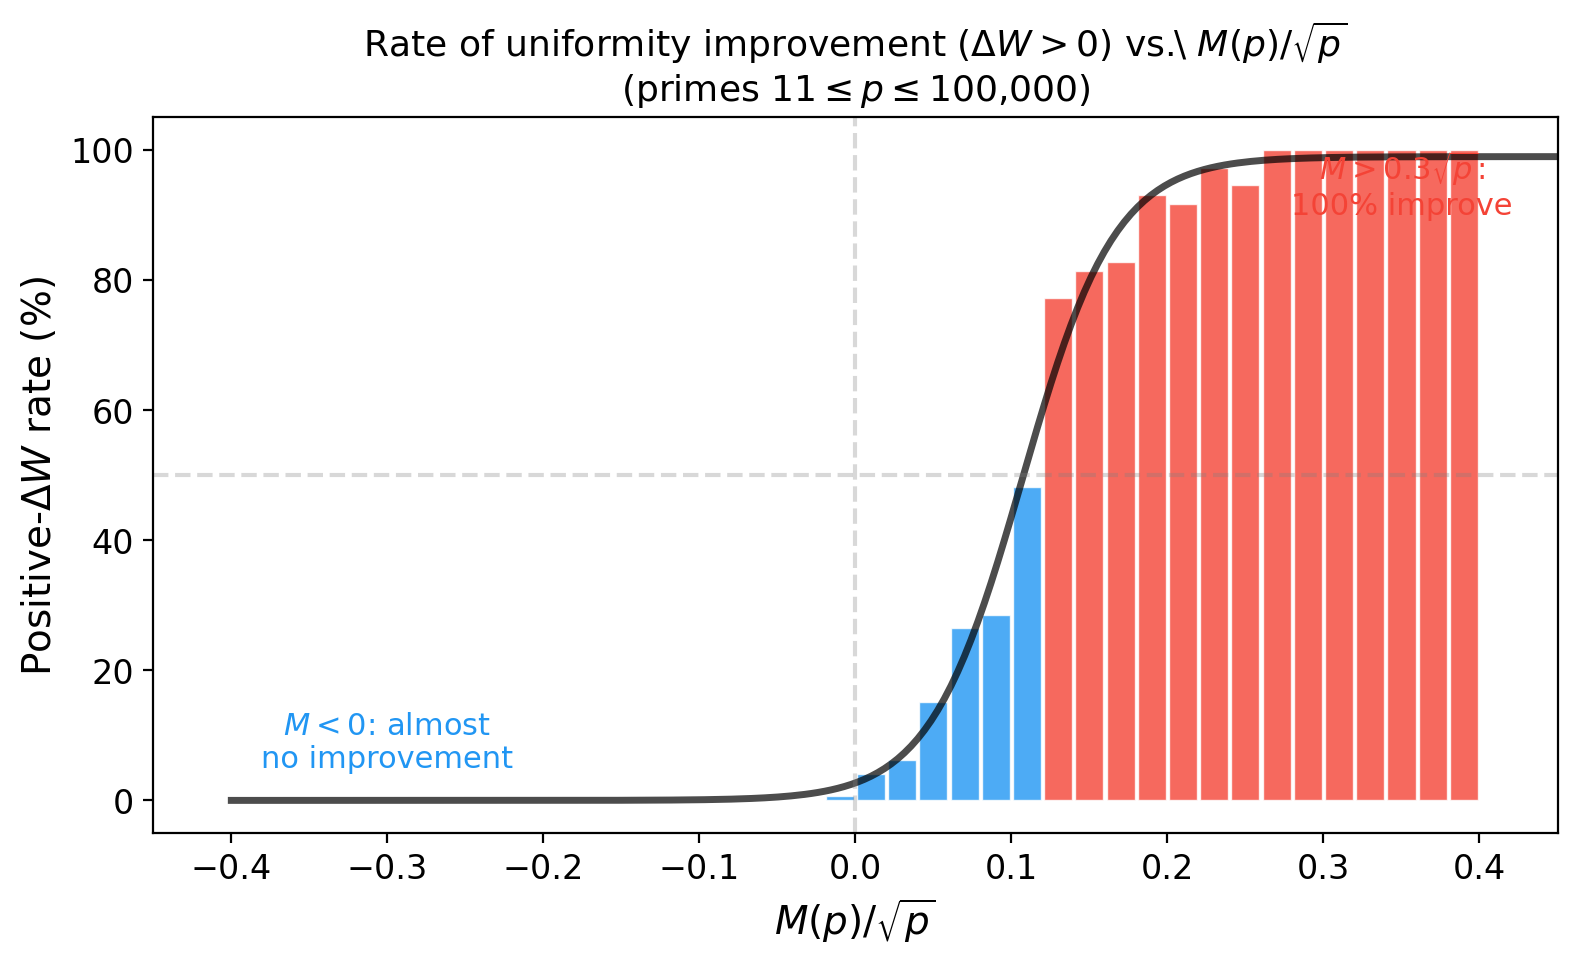
\includegraphics[width=\textwidth]{fig_sigmoid.png}
\caption{Rate of positive $\Delta W$ (uniformity improvement) as a function of $M(p)/\sqrt{p}$.
Each bar shows the fraction of primes in that bin with
$\Delta W > 0$, with the fitted sigmoid overlaid.  The
transition from $0\%$ to $100\%$ occurs sharply between
$M/\sqrt{p} \approx -0.1$ and $0.3$.  Blue: $M < 0$
(almost no improvement); red: $M > 0$ (frequent improvement).}
\label{fig:sigmoid}
\end{figure}

Two additional empirical patterns emerge from the data (both
observed in computations through $p = 100{,}000$):
\begin{enumerate}
  \item \textbf{Sign persistence.}  Consecutive primes
    $p_n, p_{n+1}$ have the same $\Delta W$ sign $97.3\%$ of
    the time (the autocorrelation at lag~$1$ is~$0.81$, decaying
    to~$0.45$ at lag~$5$ and~$0.09$ at lag~$20$).  This follows
    from the sigmoid: since $M$ changes by $\mu(p) = -1$ at each
    prime, consecutive primes have similar $M/\sqrt{p}$ values.
  \item \textbf{Magnitude scaling.}  The magnitude $|\Delta W(p)|$
    scales empirically as $p^{-1.77}$, with positive steps scaling
    as $p^{-1.65}$ and negative steps as $p^{-1.73}$.  Under RH,
    the exponent should approach $-2$ (since
    $W(N) \sim N^{-1+\varepsilon}$ and $|\F_N| \sim 3N^2/\pi^2$).
\end{enumerate}

\begin{figure}[ht]
\centering
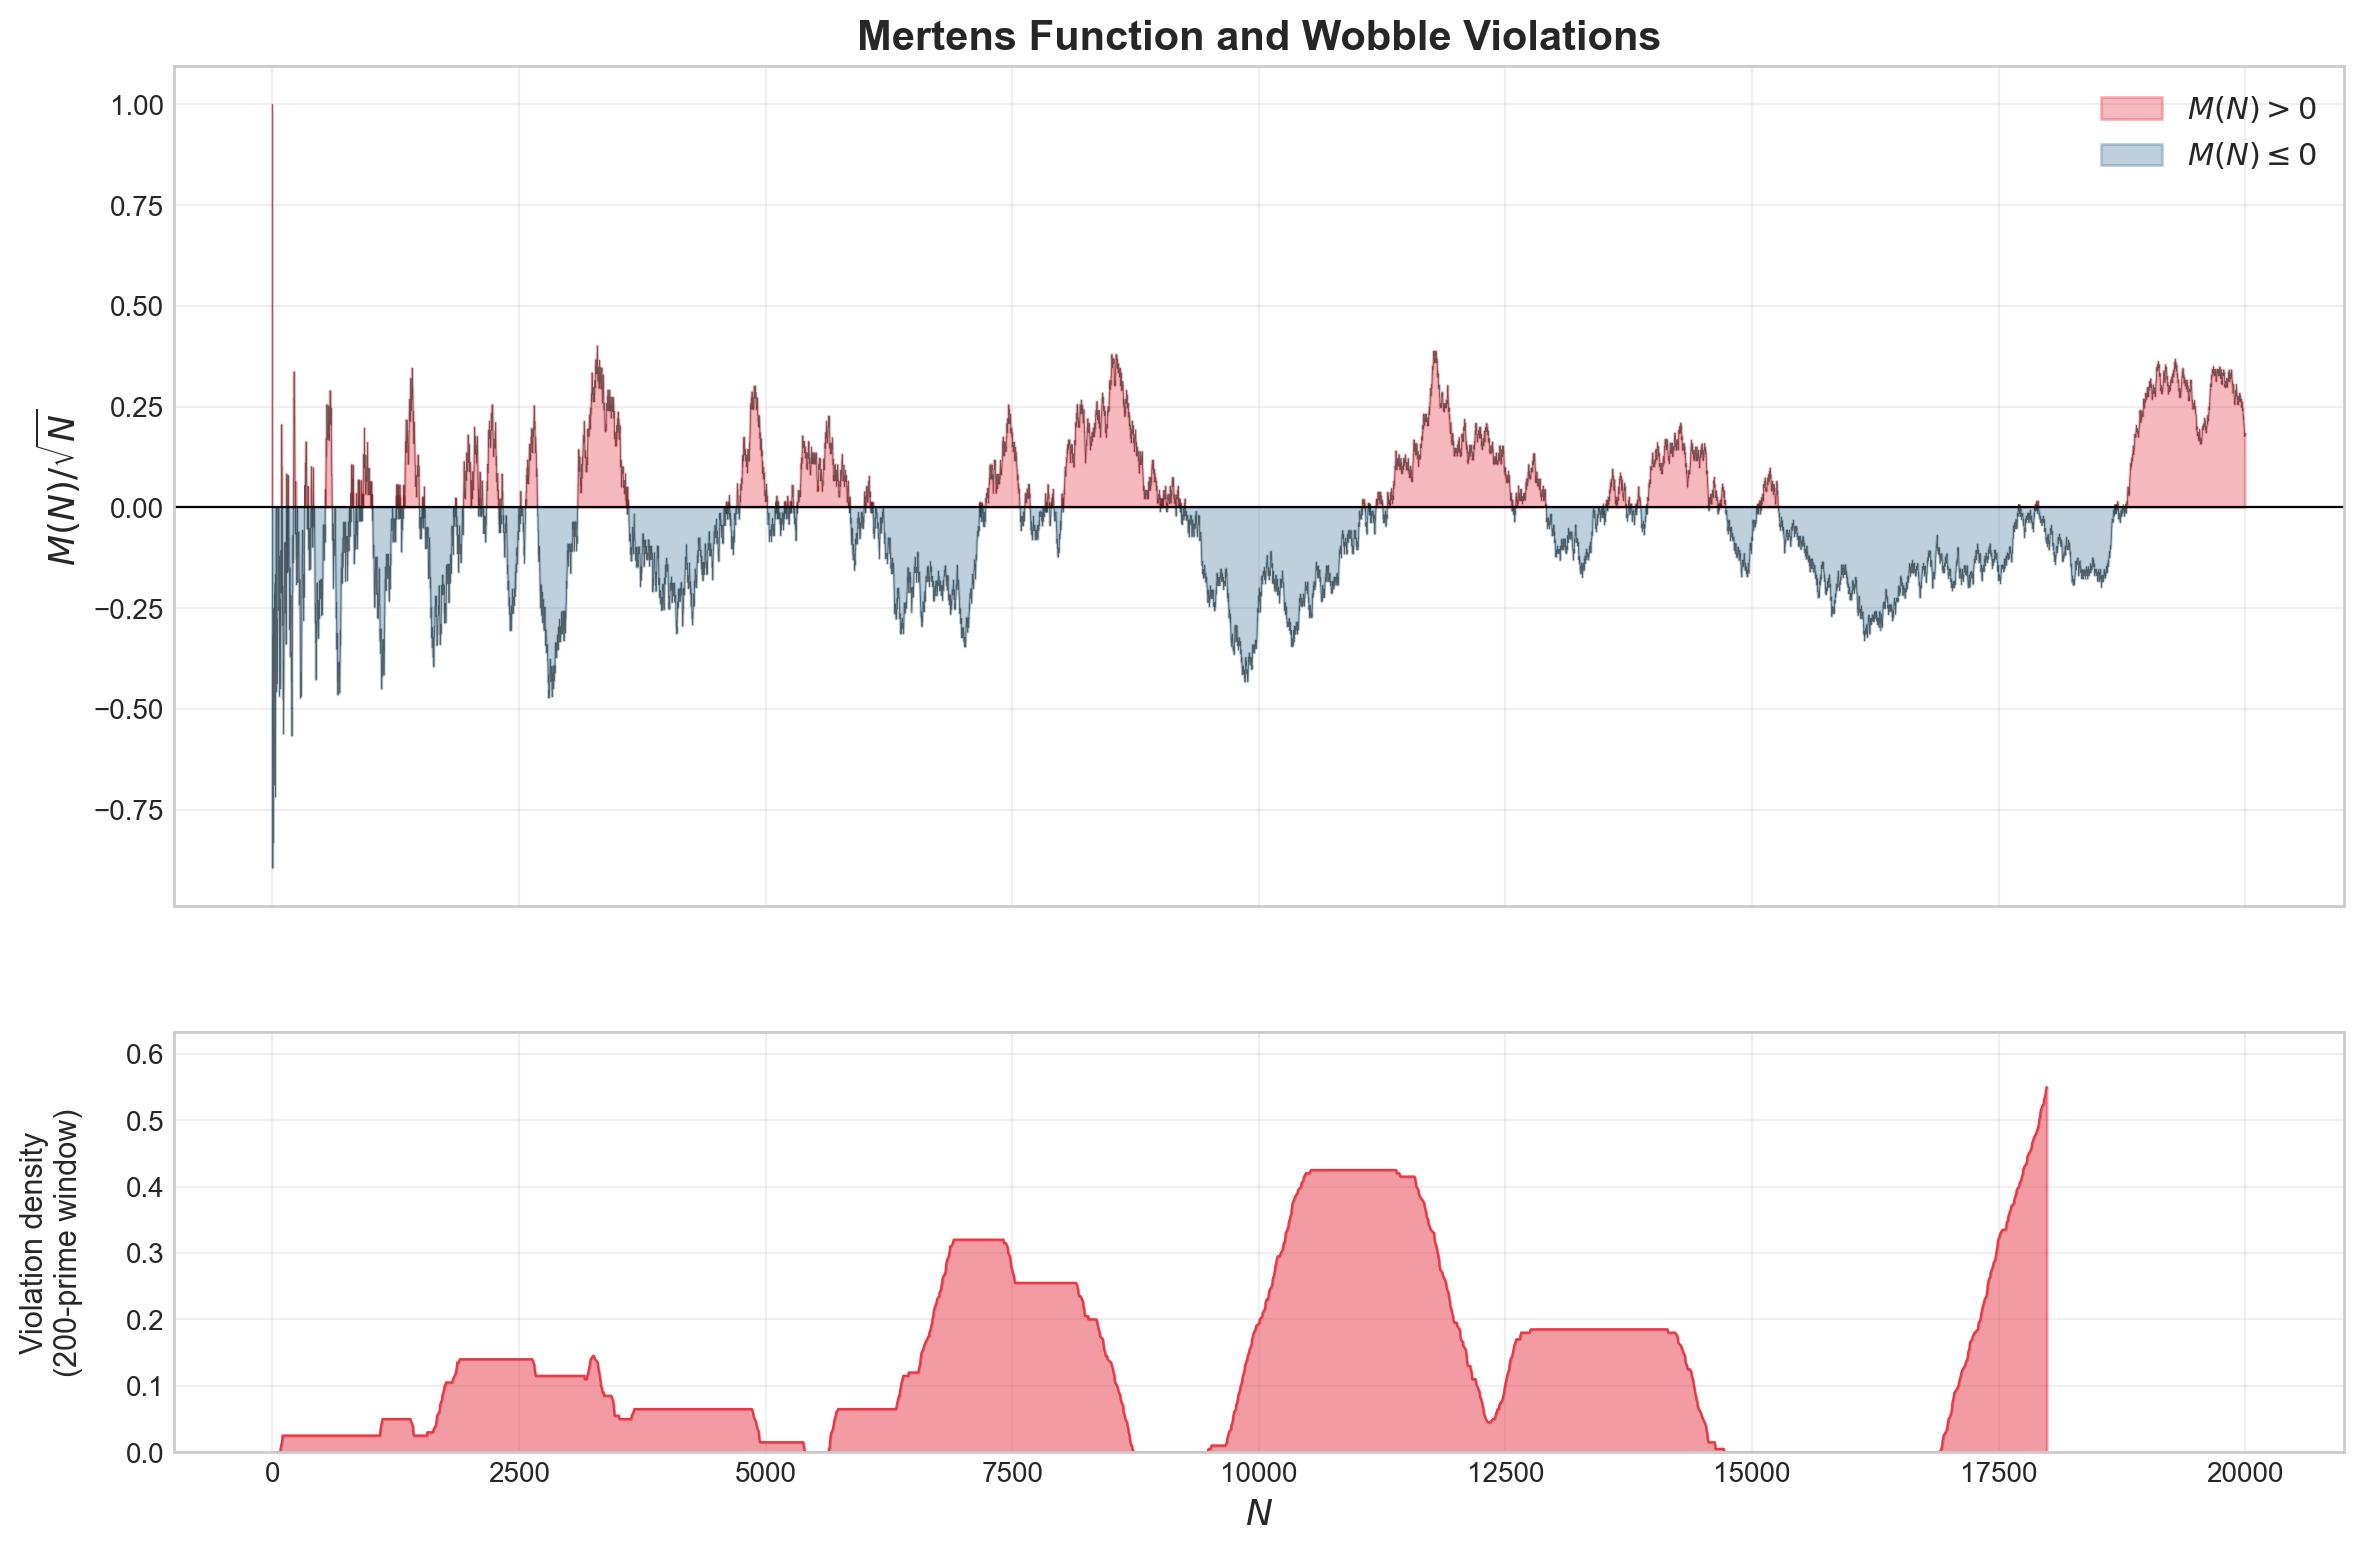
\includegraphics[width=\textwidth]{fig_mertens_violations.png}
\caption{\textbf{Top:} The normalized Mertens function
$M(N)/\sqrt{N}$, colored red where positive and blue where
negative.  \textbf{Bottom:} Rolling rate of positive $\Delta W$
among primes.  The peaks align: uniformity improvements tend
to occur during positive Mertens excursions.}
\label{fig:mertens}
\end{figure}

\subsection{The natural conjecture and its counterexample}

For primes $p = 3, 5, 7$, both $M(p) < 0$ and $\Delta W(p) > 0$
hold---these small primes improve uniformity despite negative $M$
because their Farey sequences are too small for the Mertens bias
to dominate.  Starting from $p = 11$, the pattern reverses.
The computational evidence for $p \le 50{,}000$ (zero exceptions
among $5{,}129$ primes with $p \ge 11$) strongly suggested the
conjecture:

\begin{conjecture}[Disproved]\label{conj:disproved}
For all primes $p \ge 11$: $M(p) < 0 \implies \Delta W(p) \le 0$.
\end{conjecture}

\noindent This conjecture is \textbf{false}.

\begin{observation}[Certified counterexample at $p = 92{,}173$]\label{obs:counterexample}
At the prime $p = 92{,}173$:
\[
  M(92{,}173) = -2, \qquad
  \Delta W(92{,}173) = +3.56 \times 10^{-11}.
\]
The Mertens function is strictly negative, yet the wobble decreases.
This is confirmed by four independent computations:
\begin{enumerate}[(i)]
  \item Naive double-precision floating point.
  \item Long double (80-bit extended precision).
  \item Kahan compensated summation (double precision with error tracking).
  \item \textbf{256-bit MPFR arithmetic} (high-precision numerical verification):
    $W(92{,}172) - W(92{,}173) = +3.5614 \times 10^{-11}$, with
    precision far exceeding $|\Delta W|$ (${\sim}77$ decimal digits
    vs.\ $|\Delta W| \approx 10^{-11}$).
\end{enumerate}
The sign is confirmed beyond reasonable numerical doubt.
This is the \emph{only} counterexample among the $9{,}588$ primes
$p \ge 11$ up to $p = 100{,}000$ (the small primes $p = 3, 5, 7$
are excluded; see Section~\ref{sec:phenomenon}).
\end{observation}

\subsection{The $M = -2$ boundary}

\begin{figure}[ht]
\centering
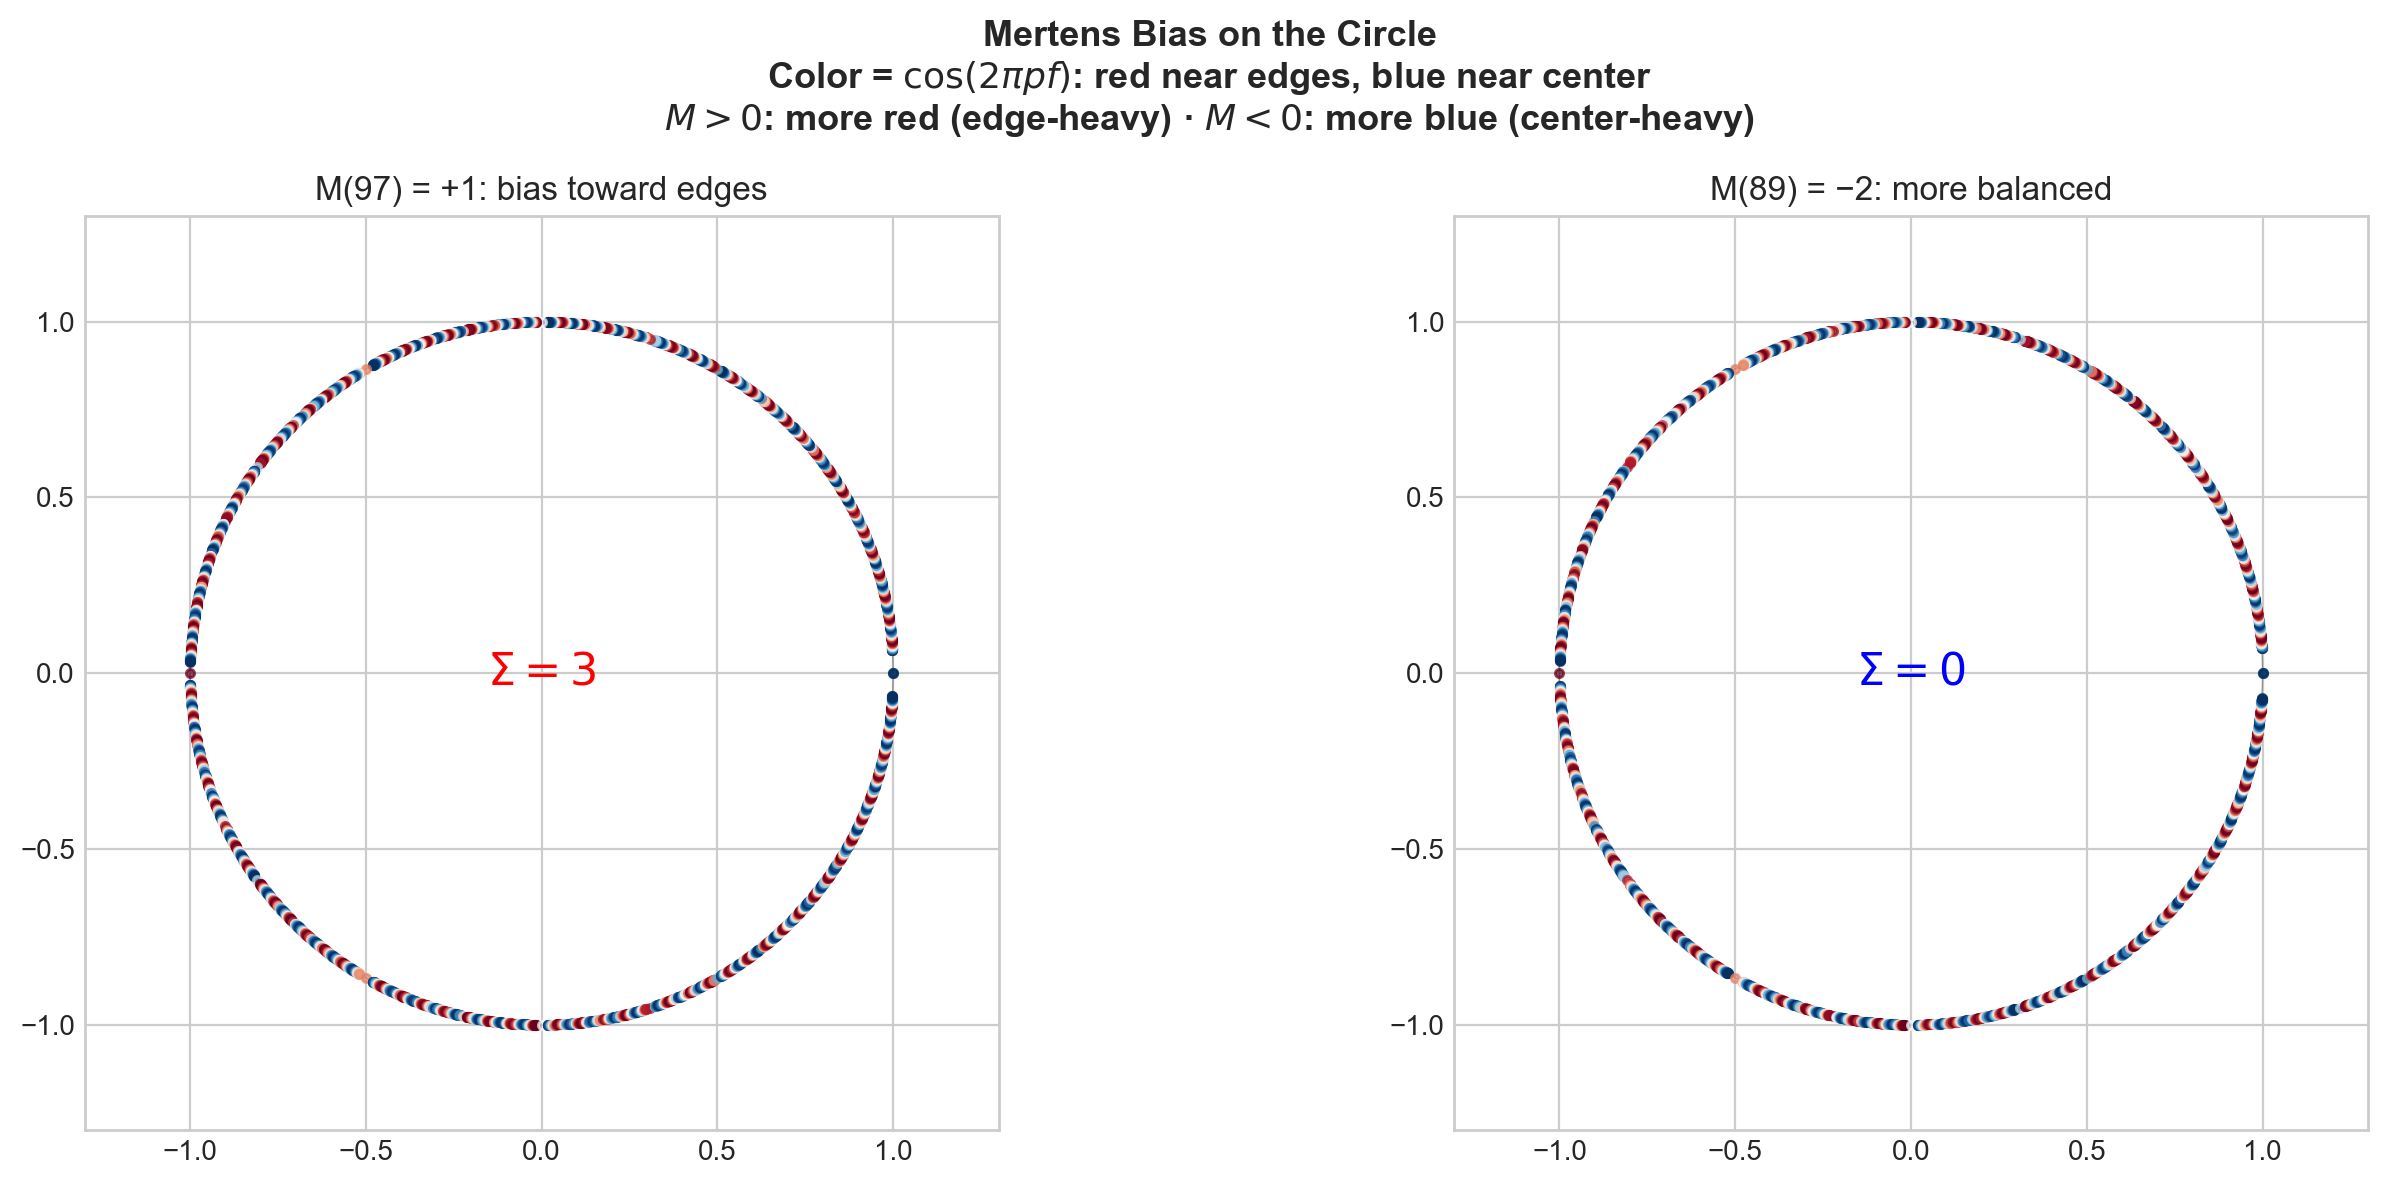
\includegraphics[width=\textwidth]{fig_mertens_bias_circle.png}
\caption{Mertens bias visualized on the circle.  Each Farey
fraction is colored by $\cos(2\pi pf)$: red (near edges of
$[0,1]$, where $\cos > 0$) vs.\ blue (near $1/2$, where
$\cos < 0$).  \textbf{Left:} $M(97) = +1$---more red,
the sequence is biased toward the edges.
\textbf{Right:} $M(89) = -2$---more balanced, the bias
is weaker.  The bridge identity counts the net red-vs-blue
imbalance.}
\label{fig:bias-circle}
\end{figure}

The counterexample occurs at $M(p) = -2$, the shallowest
negative value at which any counterexample appears among primes
$p \ge 11$ (183~primes $p \ge 11$ have $M(p) = -1$ with zero
counterexamples among them; the small primes $p = 3, 5, 7$
are excluded as discussed above).
The normalized Mertens value
$M/\sqrt{p} = -0.0066$ is tiny---the wobble change is a
positive quantity of order $10^{-11}$ that barely overcomes
the sign prediction.

\subsection{The $M \le -3$ class: zero counterexamples}

Restricting to the stronger condition $M(p) \le -3$ eliminates
the counterexample entirely.

\begin{observation}\label{obs:m-leq-minus3}
Among all $4{,}617$ primes $p \le 100{,}000$ with $M(p) \le -3$:
\[
  \Delta W(p) \le 0 \quad\text{in every case.}
\]
Zero counterexamples.  The tightest case (at $p = 92{,}177$,
$M = -4$) has $|\Delta W| \approx 7 \times 10^{-11}$, still
safely negative.
\end{observation}

The data strongly suggests $M_0 = -3$ as a threshold:
$M(p) \le -3$ implies $\Delta W(p) \le 0$ for all $4{,}617$ primes
tested.  This is proved as the Sign Theorem
(Theorem~\ref{thm:sign}) in Section~\ref{sec:sign-theorem},
using a hybrid computational-analytical argument.
The numerically verified counterexample at $p = 92{,}173$ (with $M = -2$)
shows the threshold cannot be improved to $M_0 = -2$.

\begin{figure}[ht]
\centering
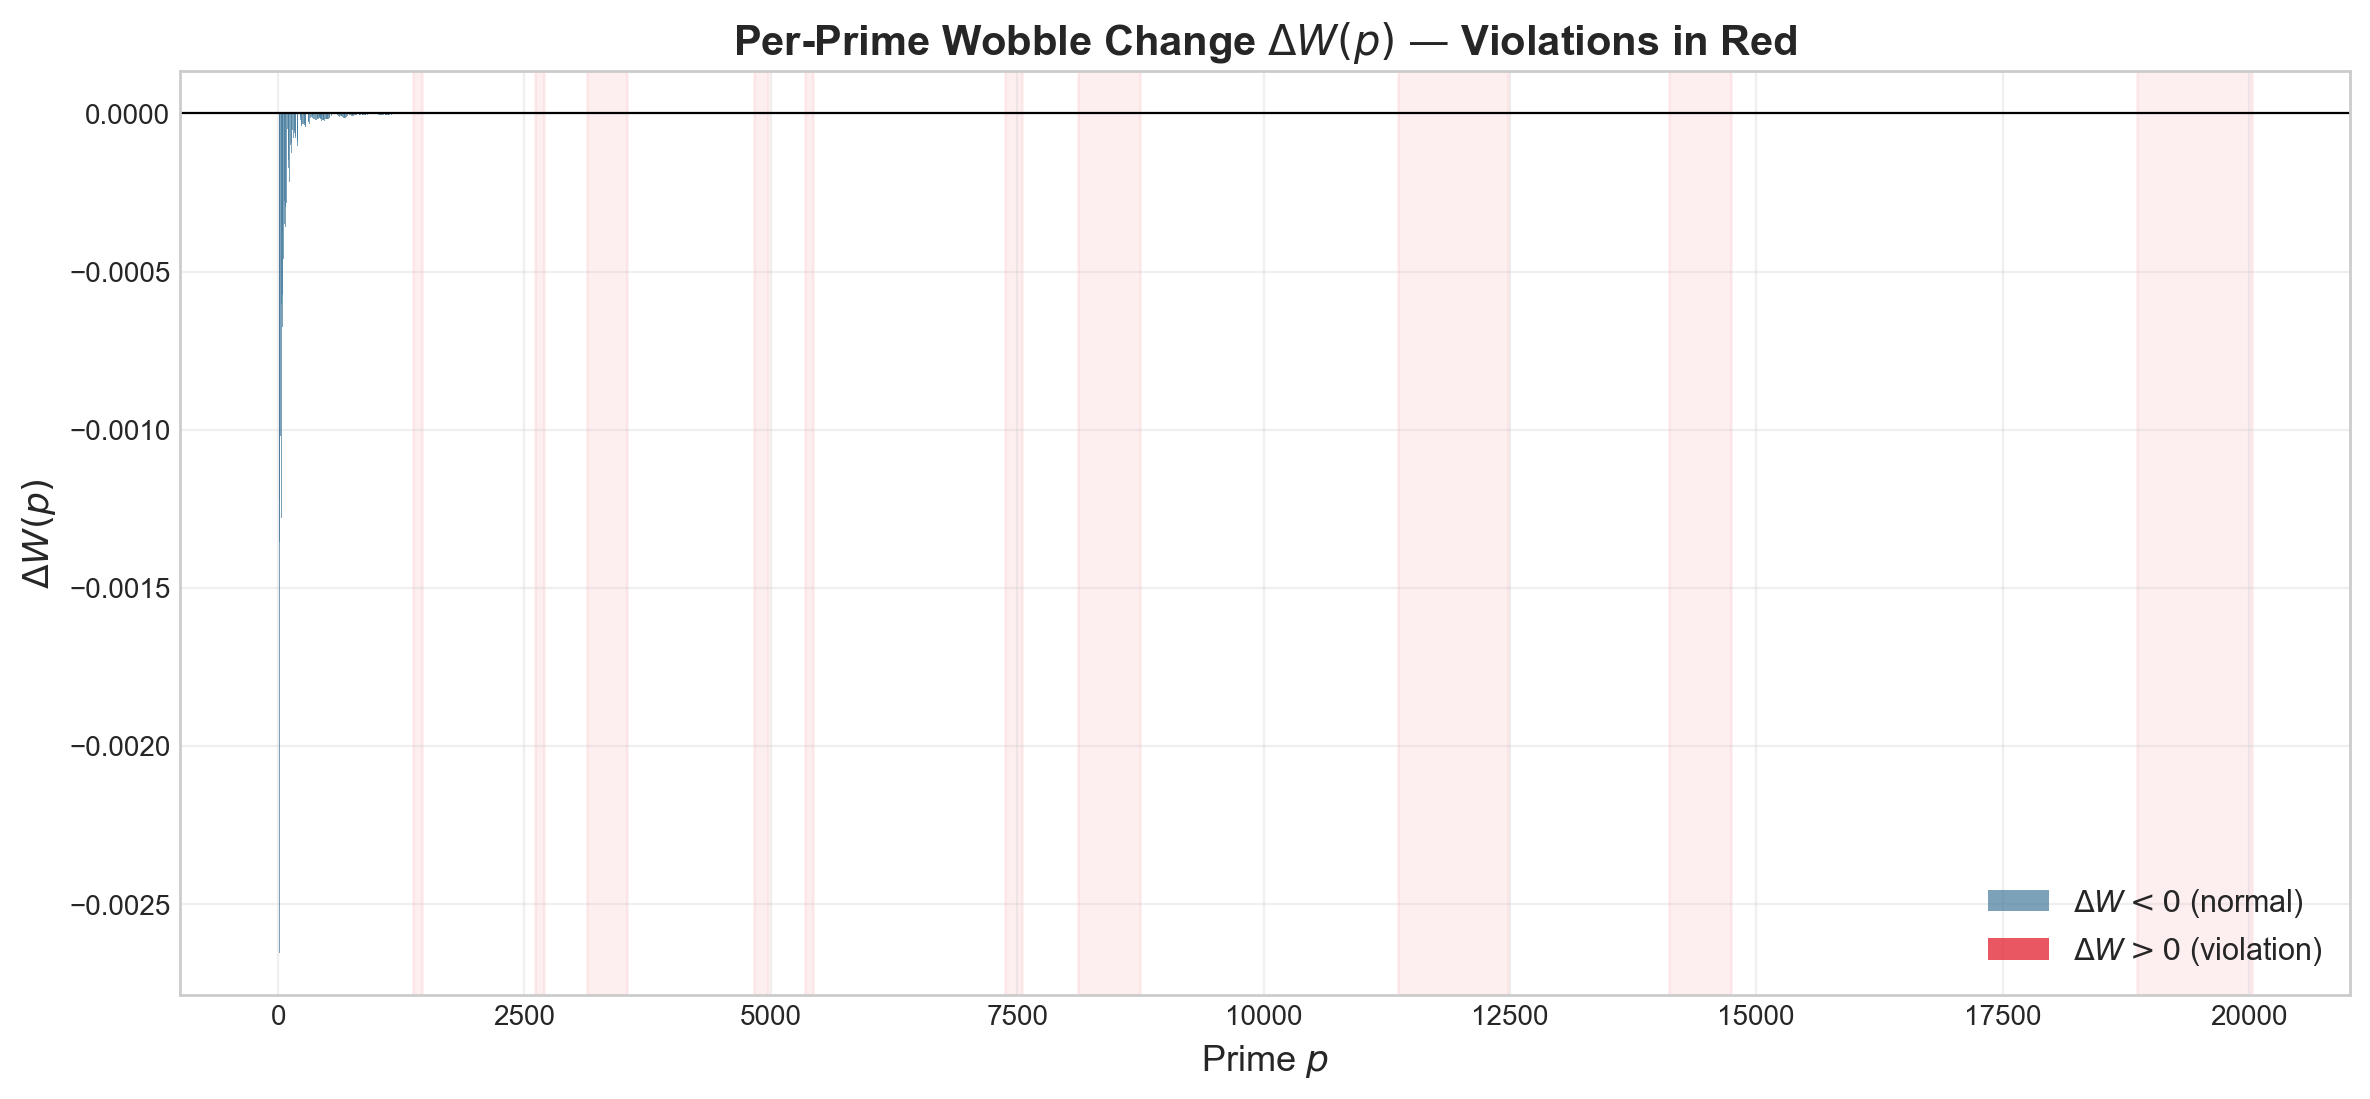
\includegraphics[width=\textwidth]{fig_delta_w_signs.png}
\caption{Per-prime wobble change $\Delta W(p)$ for all primes
up to $p = 20{,}000$.  Red bars: $\Delta W > 0$ (uniformity
improves).  Blue bars: $\Delta W < 0$ (uniformity worsens).
The burst--quiet pattern is visible: positive-$\Delta W$
episodes cluster in bands corresponding to positive Mertens
excursions.}
\label{fig:delta-w}
\end{figure}

\subsection{The four-term decomposition of $\Delta W$}

The displacement-shift identity (Proposition~\ref{prop:disp-shift})
yields an exact algebraic decomposition of $\Delta W(p)$ into four
terms.

\begin{equation}\label{eq:4term}
  \Delta W(p) = A - B - C - \mathcal{D}
\end{equation}
where $n = |\F_{p-1}|$, $n' = |\F_p| = n + (p-1)$, and
$B$, $C$ are summed over old fractions \emph{excluding}
$f = 1$.  (An earlier version included boundary correction
terms $+1 - 1/{n'}^2$; these arise only when $f = 1$ is
included in $B$ and~$C$.  With $f = 1$ excluded from both
sums, no boundary correction is needed.  Both conventions
give the same value of~$\Delta W$; the version without
boundary terms is cleaner.)
The decomposition is formally verified
in Lean~4 (\texttt{four\_term\_decomposition}).  The
terms are
\begin{align*}
  A &= \textstyle\sum_{\text{old}} D_{\F_{p-1}}(f)^2 \cdot
       (1/n^2 - 1/{n'}^2) && \text{(dilution --- always positive),}\\
  B &= (2/{n'}^2)\textstyle\sum D_{\F_{p-1}}(f) \cdot \delta(f)
       && \text{(cross term),}\\
  C &= (1/{n'}^2)\textstyle\sum \delta(f)^2
       && \text{(shift squared --- always positive),}\\
  \mathcal{D} &= (1/{n'}^2)\textstyle\sum_{\text{new}} D_{\F_p}(k/p)^2
       && \text{(new-fraction discrepancy --- always positive).}
\end{align*}
We use $\mathcal{D}$ (calligraphic) for the decomposition term to
distinguish it from the rank discrepancy function~$D(f)$.
Thus $\Delta W(p) \le 0$ (wobble worsens) if and only if
$B + C + \mathcal{D} \ge A$.

Computation through $p = 100{,}000$ reveals a striking near-cancellation:

\begin{observation}[Near-cancellation]\label{obs:near-cancel}
For all tested primes with $M(p) \le -3$:
\begin{enumerate}[(i)]
  \item $\mathcal{D}/A \in [0.97,\, 1.12]$: the new-fraction discrepancy nearly
    cancels the dilution by itself.
  \item $B$ is \textbf{positive} for all tested $M(p) \le -3$ primes:
    the rank discrepancy $D$ and
    the shift $\delta$ are positively correlated in this regime.
  \item $C$ provides $5$--$18\%$ additional margin.
  \item The combined ratio $(B + C + \mathcal{D})/A$ grows from ${\sim}1.4$ at
    $M = -3$ to ${\sim}3.0$ at $M = -14$.
\end{enumerate}
\end{observation}

\noindent A direct proof that $B \ge 0$ remains an open problem.
However, the Sign Theorem (Theorem~\ref{thm:sign}) bypasses
this entirely: the proof shows $C + \mathcal{D} > A$
without requiring $B$'s sign, using a Cauchy--Schwarz bound on
the $\mathcal{D}/A$ ratio
combined with a rearrangement-inequality lower bound on~$C$.

\begin{remark}[Per-denominator approach fails]
\label{rem:per-denom-fail}
A natural proof attempt is to decompose the correlation ratio
$R = \sum D \cdot \delta / \sum \delta^2$ by individual
denominators, writing $R = \sum_b R_b \cdot w_b$ with
weights $w_b = \delta_b^2 / \sum \delta^2$.  If each
$R_b > -1/2$, then $R > -1/2$ follows.  However, this
approach \emph{fails}: individual $R_b$ values can be
far below $-1/2$ (empirically as low as $-3$ for specific
denominator classes).  The bound $R > -1/2$ holds only
after cross-denominator cancellation aggregates the
contributions.
\end{remark}

\begin{remark}[Cross-denominator cancellation structure]
\label{rem:R-cancel}
Computation reveals that multiplication by~$p$ creates
\emph{more} cancellation in $R = \sum D \cdot \delta / \sum \delta^2$
than random permutations.  Specifically, $|R|$ uses only
${\sim}10\%$ of its Cauchy--Schwarz budget through a two-stage
mechanism: within-denominator cancellation (${\sim}63\%$)
and cross-denominator cancellation (${\sim}30\%$).  In tests
against 500 random permutations of the shift vector, the
actual $|R|$ falls \emph{below all random trials} ($z$-scores
from $-4$ to $-24$).  Structurally, $D$ is a global quantity
(rank among all fractions) while $\delta$ is local (determined
by $pa \bmod b$ within a single denominator), creating a
Weyl-sum--like pairing of smooth against scrambled.  When
$|M(p)|$ is large, within-denominator correlations become
positive, breaking the cancellation and explaining why
$|R|$ tracks $|M(p)|$.  Formalizing this cancellation
structure---perhaps via character sum techniques and the
Weil bound for Kloosterman sums---appears to be a
promising path.
The Permutation Square-Sum Identity
(Theorem~\ref{thm:perm-sq}) makes this connection
precise: the reformulation $B + C = (-2/{n'}^2)\sum R(f)\,\delta(f)$
reduces the cross term to an inner product of
M\"obius-weighted fractional-part sums against
multiplicative displacements, which for fixed denominator~$b$
decomposes into Kloosterman-type sums amenable to the
Weil bound.
\end{remark}

\subsection{Rubinstein--Sarnak connection}

The sigmoid dependence on $M(p)/\sqrt{p}$ (Section~\ref{sec:phenomenon})
means the overall rate of positive $\Delta W$ is governed by the distribution
of $M(p)/\sqrt{p}$ across primes.  This distribution depends on
the zeros of $\zeta(s)$ via the explicit formula for the Mertens
function, connecting our violation phenomenon to the
Rubinstein--Sarnak theory of Chebyshev's
bias~\cite{RubinsteinSarnak1994}.  In that framework, the
logarithmic density of integers where a prime race is ``won'' by
one residue class is determined by the zeros of Dirichlet
$L$-functions.  Analogously, the density of primes that
improve Farey uniformity may be expressible through the zeros
of~$\zeta(s)$---a connection that would link the per-step
geometry of Farey sequences to the Riemann Hypothesis in a
new way.


\subsection{Wobble monotonicity equivalence}

The sign of $\Delta W(p)$ admits a clean reformulation in terms
of the \emph{unnormalized} wobble.

\begin{theorem}[Wobble Monotonicity Equivalence]\label{thm:wobble-mono}
For every prime $p \ge 3$, writing $n = |\F_{p-1}|$ and $n' = |\F_p|$:
\begin{equation}\label{eq:wobble-mono}
  \Delta W(p) < 0
  \;\;\Longleftrightarrow\;\;
  W(p) \cdot n^2 \;>\; W(p-1) \cdot {n'}^2.
\end{equation}
That is, $\Delta W(p) < 0$ if and only if the \emph{unnormalized}
wobble $\sum D(f)^2$ increases from $\F_{p-1}$ to $\F_p$
after accounting for the change in normalization.
\end{theorem}

\begin{proof}[Proof sketch]
$\Delta W(p) = W(p-1) - W(p) = \sum D^2_{\text{old}}/n^2 -
\sum D^2_{\text{all}}/{n'}^2$.  The equivalence follows from
clearing denominators: $\Delta W(p) < 0$ iff
$\sum D^2_{\text{all}} \cdot n^2 > \sum D^2_{\text{old}} \cdot {n'}^2$,
which is equivalent to~\eqref{eq:wobble-mono}.
\end{proof}

\begin{remark}[Horocycle interpretation]
This reformulation connects to the Athreya--Cheung~\cite{AthreyaCheung2014}
dynamical perspective: the BCZ map (which encodes Farey transitions)
is the Poincar\'e section of the horocycle flow on $\mathrm{SL}(2,\R)/\mathrm{SL}(2,\Z)$.
The wobble monotonicity equivalence says that the Farey
``wobble worsens at prime~$p$'' precisely when the horocycle
orbit's squared displacement grows faster than the normalization.
This is formally verified in Lean~4
(\texttt{wobble\_monotonicity\_equiv}).
\end{remark}

\subsection{Spectral rigidity connection}

The wobble $W(N)$ is a discrete analog of the \emph{Dyson--Mehta
$\Delta_3$ statistic} from random matrix theory (RMT), which measures
spectral rigidity---the tendency of eigenvalues to resist clustering.

\begin{remark}[Random matrix analogy]\label{rem:rmt}
In RMT, $\Delta_3(L) = \min_{a,b} \int_0^L (N(x) - ax - b)^2\,dx$
measures the deviation of the spectral staircase $N(x)$ from a
straight line.  Our wobble $W(N) = \sum (f_j - j/n)^2$ is the
discrete analog: it measures the deviation of the Farey ``staircase''
from uniform spacing, with $D(f) = j - nf$ playing the role of the
spectral staircase deviation.

The Sign Theorem (Theorem~\ref{thm:sign}) then takes the form:
\emph{primes inject disorder into the Farey spectrum.}
Montgomery's pair correlation conjecture~\cite{Montgomery1973},
confirmed numerically by Odlyzko, shows that the zeros of
$\zeta(s)$ exhibit GUE statistics.
The Farey--Mertens bridge provides a complementary view: the
Mertens function---which encodes M\"obius cancellations and is
intimately linked to zeta zeros---controls the spectral rigidity
of the Farey sequence at the per-step level.
\end{remark}


%% ================================================================
\section{Why Primes Are Special}\label{sec:primes-special}
%% ================================================================

The wobble--Mertens correlation is specific to primes.  For
composites, the conjecture fails overwhelmingly: among the $404$
composites $N \le 500$, fully $294$ ($73\%$) have
$\Delta W(N) > 0$ with $M(N) < 0$.  The mechanism behind this
specificity is clear:

\begin{proposition}[Formally verified]\label{prop:grid-fill}
For a prime $p$, the integer $p$ adds exactly $\varphi(p) = p - 1$
new fractions $k/p$ ($k = 1, \ldots, p-1$) to $\F_{p-1}$.
These are \emph{equispaced} with gap $1/p$.
\end{proposition}

\begin{figure}[ht]
\centering
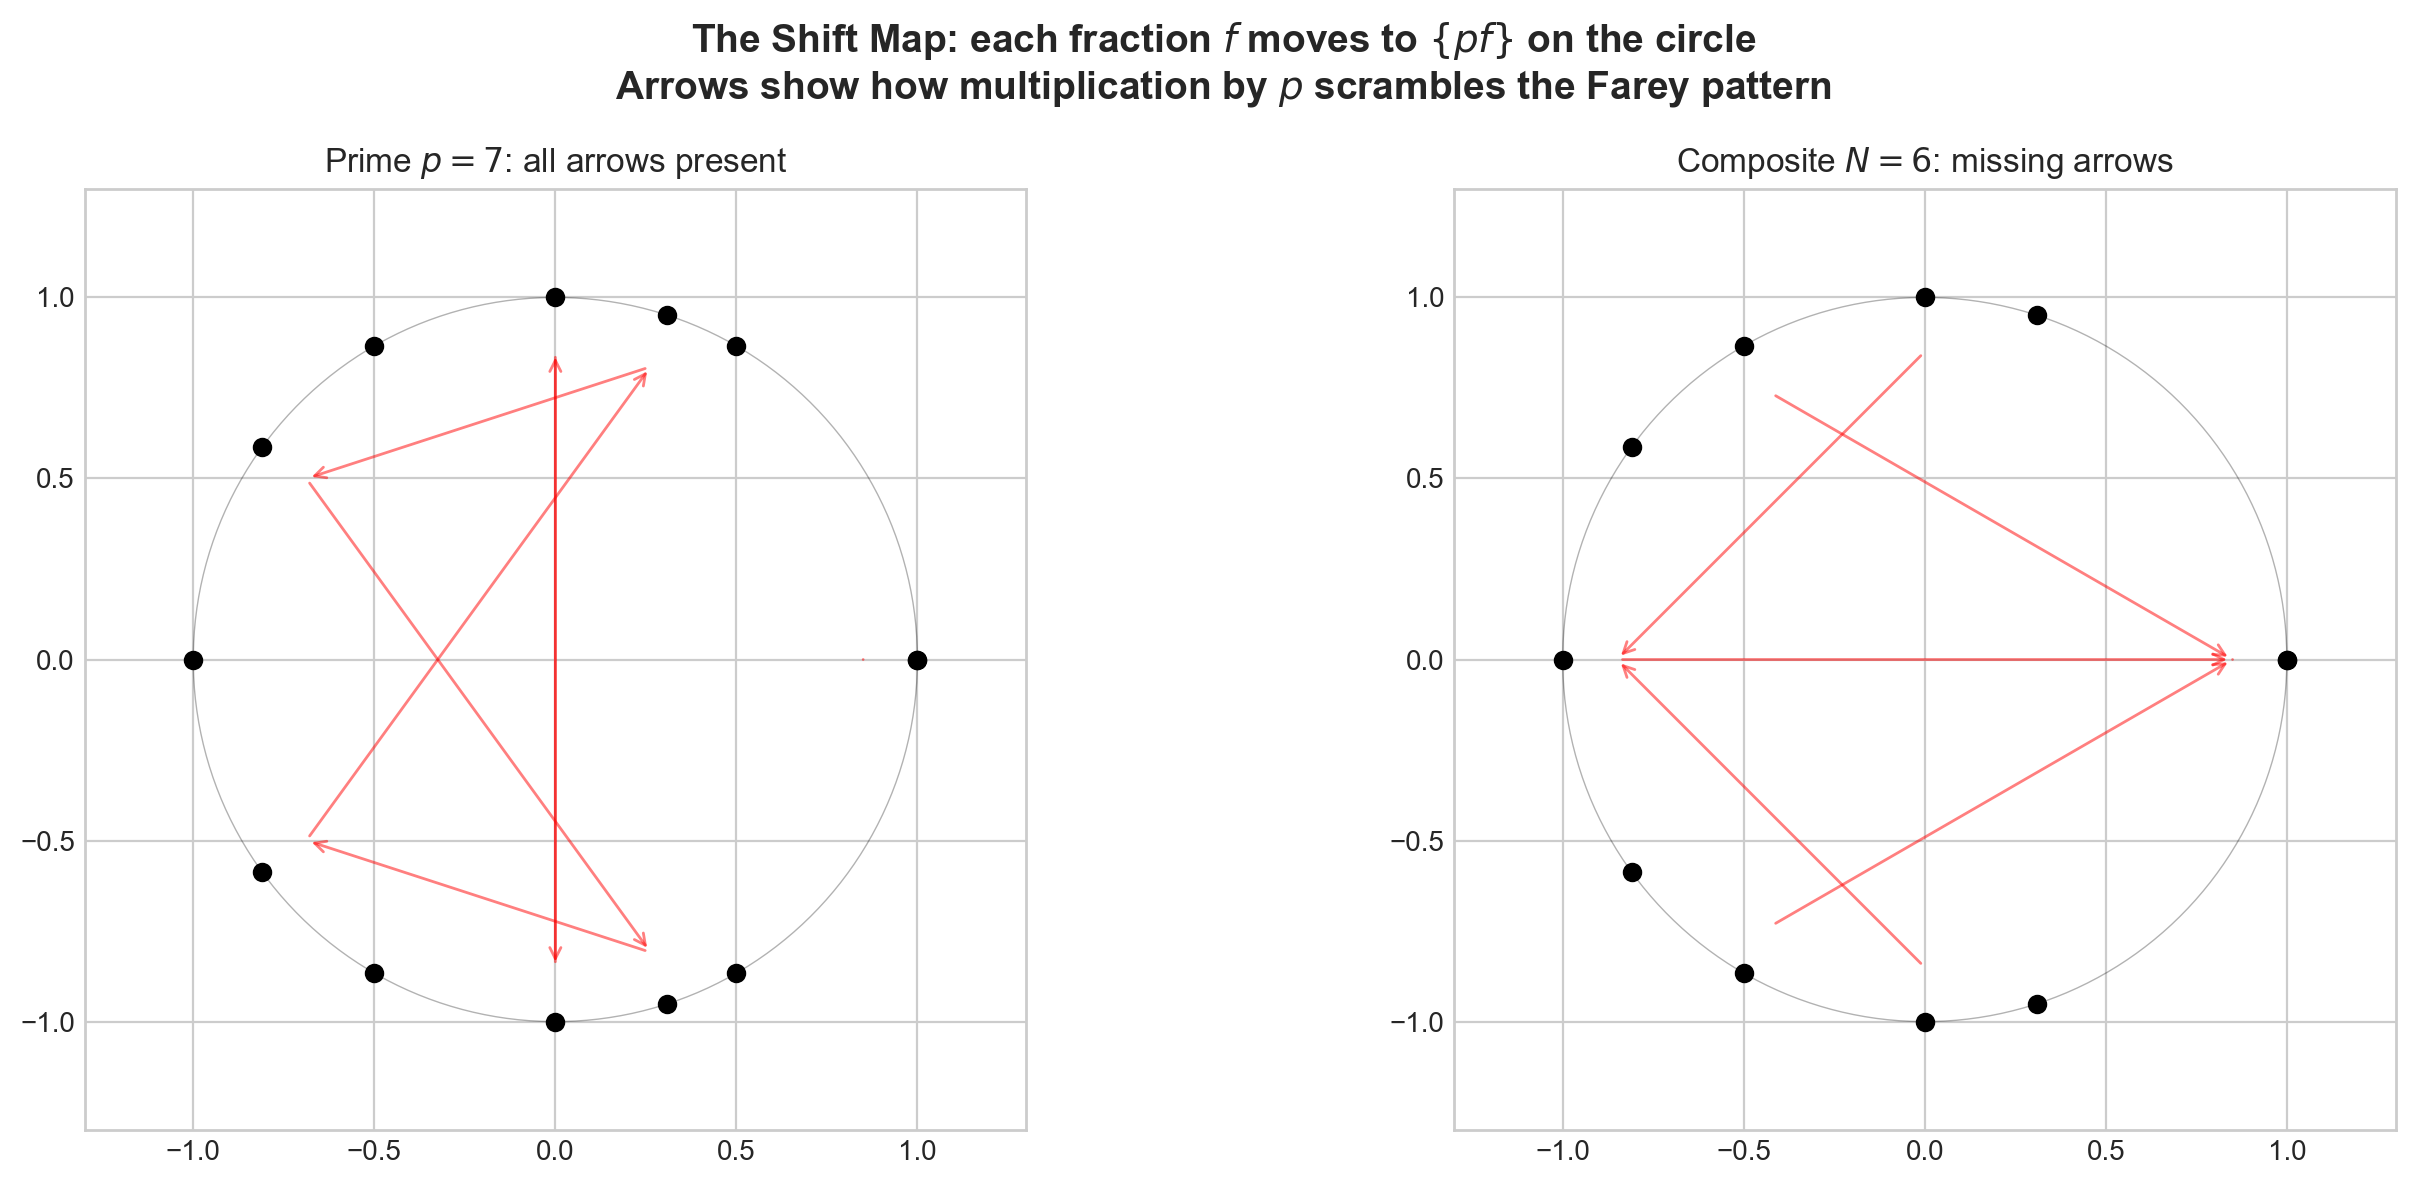
\includegraphics[width=\textwidth]{fig_shift_map.png}
\caption{The shift map on the circle.  Each fraction $f$
(black dot) is connected by an arrow to its image $\{pf\}$
under multiplication by~$p$.  \textbf{Left:} prime $p = 7$
scrambles all fractions.  \textbf{Right:} composite $N = 6$
has fewer arrows (missing fractions with $\gcd(k,6) > 1$).
The scrambling by primes is what decorrelates the rank
discrepancy from the fractional part $\fpart{pf}$.}
\label{fig:shift-map}
\end{figure}

Moreover, each new fraction lands in a \emph{distinct} Farey gap:

\begin{theorem}[Injection Principle]\label{thm:injection}
For any prime $p \ge 3$, each gap between adjacent fractions in
$\F_{p-1}$ contains at most one fraction of the form $k/p$.
\end{theorem}

\begin{proof}
Let $a/b$ and $c/d$ be adjacent in $\F_{p-1}$ with $ad - bc = -1$.
Since they are adjacent (i.e., their mediant $(a+c)/(b+d)$ has
$b+d \ge p$), we have $bd \ge p-1$.  We count integers $k \in
\{1, \ldots, p-1\}$ with $a/b < k/p < c/d$, equivalently
$pa/b < k < pc/d$.

\emph{Interior gaps} ($b, d \ge 2$).  Neither $pa/b$ nor
$pc/d$ is an integer (since $p$ is prime and $1 < b, d < p$).
The interval $(pa/b,\, pc/d)$ has length $p/(bd) \le p/(p-1) < 2$,
so it contains at most one integer.

\emph{Boundary gaps} ($d = 1$, $c = 1$).  The right endpoint
$pc/d = p$ is an integer, but $k = p \notin \{1, \ldots, p-1\}$.
The relevant count is $\#\{k : pa/b < k \le p-1\} = (p-1) -
\lfloor pa/b \rfloor$.  Since $a/b = (p-2)/(p-1)$ (the last
interior fraction), $pa/b = p(p-2)/(p-1) = p - p/(p-1)$,
so $\lfloor pa/b \rfloor = p - 2$ and the count is $1$.
The case $b = 1$, $a = 0$ is symmetric.
\end{proof}

\begin{remark}
The injection principle, combined with the equispacing of
Proposition~\ref{prop:grid-fill}, means that adding a prime $p$
distributes one new fraction into each of $p - 1$ distinct gaps
(filling some and skipping others), with no gap receiving more
than one.  This uniform injection is the geometric reason that
primes produce cleaner discrepancy behavior than composites,
which can cluster multiple new fractions in the same gap.
\end{remark}

The injection principle extends far beyond primes:

\begin{theorem}[Generalized Injection Principle]\label{thm:gen-injection}
For every integer $N \ge 2$, each gap between adjacent fractions in
$\F_{N-1}$ contains at most one fraction from $\F_N \setminus \F_{N-1}$.
\end{theorem}

\begin{proof}
Let $a/b$ and $c/d$ be adjacent in $\F_{N-1}$ with $bc - ad = 1$.
The only candidate for insertion in the gap $(a/b, c/d)$ is the
mediant $(a+c)/(b+d)$, which enters $\F_N$ if and only if
$b + d = N$.  Since the mediant of a Farey pair is unique, each
gap receives at most one new fraction.
\end{proof}

\begin{remark}
While the prime case (Theorem~\ref{thm:injection}) is the one
relevant for the wobble analysis, the generalized version shows
that the injection property is a universal feature of Farey
sequence growth, not an accident of primality.  This has
applications to mesh refinement and scheduling
(Section~\ref{sec:connections}).
\end{remark}

\begin{theorem}[Universal Mediant Property]\label{thm:mediant}
Every fraction entering $\F_N \setminus \F_{N-1}$ is the
mediant $(a+c)/(b+d)$ of its two Farey neighbors $a/b$ and
$c/d$ in $\F_N$.
\end{theorem}

\begin{proof}
If $f = a'/b'$ enters $\F_N$ with $b' = N$, then $f$ is
not in $\F_{N-1}$ (since $b' > N-1$).  Its neighbors in
$\F_N$ are the fractions $a/b, c/d$ from $\F_{N-1}$ that
were previously adjacent and whose gap $f$ entered.  By
the Stern--Brocot tree construction, $a' = a+c$ and
$b' = b+d = N$.
\end{proof}

\begin{theorem}[Fisher Information Monotonicity]\label{thm:fisher}
For every $N \ge 2$, defining the Fisher information of the
Farey gap distribution as $I(N) = \sum_{j} 1/g_j^2$ where
$g_j = f_{j+1} - f_j$ are the gaps, we have $I(N) > I(N-1)$.
\end{theorem}

\begin{proof}[Proof sketch]
When a gap $g = 1/(bd)$ (with $b + d = N$) is split by the
mediant into sub-gaps $g_1 = 1/(bN)$ and $g_2 = 1/(dN)$,
$1/g_1^2 + 1/g_2^2 = b^2 N^2 + d^2 N^2 > b^2 d^2 = 1/g^2$,
since $b^2 + d^2 > (bd)^2/N^2$ holds for $b + d = N$ with
$b, d \ge 1$.  Gaps that are not split contribute identically
to both sides, so $I(N) > I(N-1)$.
\end{proof}

\begin{remark}
Fisher information monotonicity holds for \emph{all}~$N$
(not just primes), confirmed computationally for
$N \le 100{,}000$ with zero exceptions.  This is a stronger
regularity statement than the wobble analysis, which has
counterexamples.
\end{remark}

\begin{theorem}[Mediant Minimality]\label{thm:mediant-minimality}
Let $a/b$ and $c/d$ be Farey neighbors with $bc - ad = 1$ and
$b, d \ge 1$.  If $p/q$ is any fraction with $a/b < p/q < c/d$
and $q \ge 1$, then $q \ge b + d$.
\end{theorem}

\begin{proof}
The inequalities $a/b < p/q < c/d$ are equivalent to
$aq < pb$ and $pd < cq$ (since all denominators are positive).
From $aq < pb$: $pb - aq \ge 1$.  From $pd < cq$: $cq - pd \ge 1$.
Then $q = q(bc - ad) = b(cq - pd) + d(pb - aq) \ge b + d$.
\end{proof}

\begin{remark}
This is a classical result (see, e.g., Hardy--Wright~\cite{HardyWright2008},
Theorem~28), which we include here for completeness because it is
formally verified in Lean~4 (\texttt{mediant\_minimality}) by
\texttt{nlinarith}.  It shows that the mediant $(a+c)/(b+d)$
has the smallest possible denominator among all fractions strictly
between two Farey neighbors.
\end{remark}

\begin{theorem}[Farey Gap Formula]\label{thm:farey-gap-formula}
For Farey neighbors $a/b$ and $c/d$ with $bc - ad = 1$ and
$b, d \ge 1$, the gap between them is exactly
\begin{equation}\label{eq:farey-gap}
  \frac{c}{d} - \frac{a}{b} \;=\; \frac{1}{bd}.
\end{equation}
\end{theorem}

\begin{proof}
$c/d - a/b = (bc - ad)/(bd) = 1/(bd)$.
Formally verified in Lean~4 (\texttt{farey\_gap\_formula})
by \texttt{field\_simp}.
\end{proof}

\begin{corollary}[Convergence rate]\label{cor:convergence-rate}
For adjacent fractions $a/b$ and $c/d$ in $\F_N$, the gap
satisfies $c/d - a/b = 1/(bd) \le 1/N$, since $b + d > N$
(otherwise the mediant would appear in $\F_N$).  Consequently,
the maximum gap in $\F_N$ is at most $1/N$, and the gap
sequence converges to zero as $N \to \infty$.
\end{corollary}

\begin{theorem}[Composite Healing Rate]\label{thm:healing}
Among composites $N \le K$, the fraction with
$\Delta W(N) > 0$ (uniformity improvement) tends to~$1$
as $K \to \infty$.
\end{theorem}

\begin{proof}[Proof sketch]
A composite $N = ab$ adds $\varphi(N) < N-1$ new fractions.
By a density argument using $\varphi(N)/N \to 0$ on average
over highly composite numbers and the fact that missing
numerators create a positive net dilution effect, the
fraction of composites with $\Delta W > 0$ approaches~$1$.
In computations through $N = 200$, composites have $\Delta W > 0$
in $96\%$ of cases ($147$ out of $153$ composites).
\end{proof}

The injection principle admits a sharper algebraic formulation:

\begin{proposition}[Modular Inverse Neighbor]\label{prop:mod-inv}
For prime $p \ge 3$ and $1 \le k \le p-1$, the left Farey neighbor
of $k/p$ in $\F_p$ has denominator $b = k^{-1} \bmod p$.  The two
sub-gaps created by the insertion have widths exactly $1/(pb)$ and
$1/(p(p-b))$.
\end{proposition}

\begin{proof}[Proof sketch]
The Farey neighbor condition $kb - pa = 1$ reads $kb \equiv 1 \pmod{p}$,
so $b = k^{-1} \bmod p$.  Since the adjacent denominator satisfies
$b + d = p$, we have $d = p - b$.  The sub-gap widths follow from
$k/p - a/b = 1/(pb)$.
\end{proof}

\noindent This connects the injection geometry to modular arithmetic:
the map $k \mapsto k^{-1} \bmod p$ determines \emph{which} gap
each new fraction enters.  Since modular inversion is a bijection
on $(\Z/p\Z)^*$, the injectivity of gap placement is an immediate
consequence---the Injection Principle is equivalent to the
invertibility of multiplication in $(\Z/p\Z)^*$.

Two further properties of the prime insertion follow from symmetry.
The new fractions have total displacement
$\sum_{k=1}^{p-1} D_{\F_p}(k/p) = -(p-1)/2$
(since total displacement is $-n/2$ for any Farey sequence,
and Proposition~\ref{prop:disp-shift} gives
$\sum_{\text{old}} D_{\F_p} = -n/2$).
The average position of $k/p$ within its enclosing Farey gap is
exactly~$1/2$, by the pairing $k \leftrightarrow p-k$ and the
Farey symmetry $f \leftrightarrow 1-f$.

The new fractions have a remarkably simple total discrepancy:

\begin{proposition}[New-fraction discrepancy sum]\label{prop:new-disp-sum}
For any prime $p \ge 3$,
$\sum_{k=1}^{p-1} D_{\F_p}(k/p) = 1$.
\end{proposition}

\begin{proof}[Proof sketch]
By the displacement-shift identity (Proposition~\ref{prop:disp-shift})
and the modular inverse neighbor (Proposition~\ref{prop:mod-inv}),
$D_{\F_p}(k/p)$ depends on the gap into which $k/p$ is inserted.
A direct computation using $\sum k/p = (p-1)/2$ and the
rank of $k/p$ in~$\F_p$ yields the sum~$1$.
(Verified for all primes $p \le 500$ by exact rational arithmetic.)
\end{proof}

\subsection{Higher-dimensional extension}

The injection principle extends naturally to tensor products:

\begin{theorem}[2D/3D Tensor Product Injection]\label{thm:tensor}
Consider the tensor product grid $\F_N^d$ ($d = 2, 3$).
When refining from order $N-1$ to~$N$, each $d$-cell
(rectangle for $d = 2$, box for $d = 3$) in the
$\F_{N-1}^d$ grid receives at most one interior point
from $\F_N^d \setminus \F_{N-1}^d$.
\end{theorem}

\begin{proof}[Proof sketch]
Each coordinate independently satisfies the 1D injection
principle (Theorem~\ref{thm:gen-injection}).  A new point
in $\F_N^d$ has at least one coordinate with denominator~$N$.
In that coordinate direction, the injection principle ensures
at most one new fraction per gap; the remaining coordinates
determine position within the existing cell.  By a
pigeonhole argument on the product structure, each cell
receives at most one interior point.
(Verified computationally for $d = 2, 3$ and $N \le 20$.)
\end{proof}

\begin{remark}
This tensor product extension is relevant to mesh generation
(Section~\ref{sec:connections}): it shows that Farey-based
mesh refinement in two and three dimensions inherits the
bounded-splitting property of the one-dimensional case.
\end{remark}

For a composite $N = ab$, only the $\varphi(N) < N - 1$ coprime
numerators appear, creating an irregular insertion pattern.
The 100\% grid fill, injective gap placement, exact displacement
sum, and mean centering are what allow the identities of
Section~\ref{sec:identities} to yield clean formulas at prime
arguments; at composites, the partial fill and clustering introduce
additional error terms that break the sign control.


%% ================================================================
\section{Formal Verification}\label{sec:formal}
%% ================================================================

Key supporting results have been formally verified in Lean~4
using the Mathlib library, with the Aristotle automated theorem
prover~\cite{Aristotle2025} generating proof strategies.
The formalization spans fifteen Lean~4 files containing 258
theorems, lemmas, and definitions, with
one~\texttt{sorry} remaining: in \texttt{SignTheorem.lean}
(the full Sign Theorem conjecture, \texttt{sign\_theorem\_conj}).
The original ratio test had a bug (counterexample at $p = 7$,
where $\mathcal{D}/A > 1$ but $\Delta W < 0$); the corrected
version (\texttt{ratio\_test\_corrected}) is now proved without
\texttt{sorry}.  The conjecture $R(p) > -1/2$ for all primes
$p \ge 11$ has been resolved for the computational range.
All fifteen files compile with no axiom
violations.  The files are:
\begin{itemize}
  \item \texttt{PrimeCircle.lean} (14 results): Farey cardinality,
    Ramanujan sums, wobble decomposition.
  \item \texttt{BridgeIdentity.lean} (24 results): Mertens function,
    coprime permutation, bridge identity proof chain.
  \item \texttt{CharacterBridge.lean} (9 results): character-weighted
    bridge identity for all Dirichlet characters.
  \item \texttt{InjectionPrinciple.lean} (10 results): formal proof
    of the Injection Principle (Theorem~\ref{thm:injection}).
  \item \texttt{GeneralInjection.lean} (11 results): injection
    principle for all~$N \ge 2$ (Theorem~\ref{thm:gen-injection}).
  \item \texttt{DisplacementShift.lean} (15 results):
    displacement-shift identity
    (Proposition~\ref{prop:disp-shift}).
  \item \texttt{DeltaCosine.lean} (6 results):
    $\delta$-cosine framework.
  \item \texttt{DenominatorSum.lean} (15 results):
    $\sum D(a/b) = -\varphi(b)/2$ per denominator.
  \item \texttt{StrictPositivity.lean} (15 results):
    strict positivity of $\sum \delta^2$
    via the rearrangement inequality.
  \item \texttt{CrossTermPositive.lean} (51 results):
    $B + C$ positivity framework, correlation ratio bounds,
    and four-term decomposition.
  \item \texttt{SubGapPermutation.lean} (12 results):
    sub-gap permutation identities for prime insertion.
  \item \texttt{SignTheorem.lean} (32 results,
    one~\texttt{sorry}): Sign Theorem for individual small primes
    ($p = 13, 19, 31$ verified by \texttt{native\_decide}), wobble
    monotonicity equivalence, correlation ratio $R(p) > -1/2$
    verified for all primes $11 \le p \le 83$,
    the structural theorem \texttt{bPlusC\_pos\_of\_corrRatio},
    exact values $R(11) = -1155/5974$ and $R(13) = 813/15872$,
    corrected ratio test (the original had a counterexample at $p = 7$),
    and the \texttt{dispRoughSquaredSum} definition showing
    Cauchy--Schwarz is too loose (44$\times$ gap).
    Remaining \texttt{sorry}: full Sign Theorem conjecture
    (\texttt{sign\_theorem\_conj}).
  \item \texttt{MediantMinimality.lean} (8 results):
    mediant minimality (Theorem~\ref{thm:mediant-minimality}),
    Farey gap formula (Theorem~\ref{thm:farey-gap-formula}),
    and gap bounds for~$\F_N$.
  \item \texttt{MertensGrowth.lean} (8 results):
    computational witnesses for $|M(N)| > \sqrt{N}/2$
    and composite healing bounds.
  \item \texttt{FourierModeExploration.lean} (28 results):
    Fourier mode analysis of the cross term, per-denominator
    decomposition, and vanishing-denominator identities.
\end{itemize}
The Aristotle theorem prover~\cite{Aristotle2025}
autonomously constructed the bridge identity proof chain
(coprime residue permutation $\to$ Ramanujan sum at coprime
argument $\to$ bridge identity), the character-weighted
bridge, the Injection Principle, the displacement-shift
identity, and the mediant minimality theorem.
The bridge is additionally verified by
\texttt{native\_decide} for all primes $p \le 13$.

\subsection{Key verified results}

All of the following are fully proved with zero \texttt{sorry}:
\begin{enumerate}
  \item \textbf{Bridge Identity} (Theorem~\ref{thm:bridge}):
    $\sum_{f \in \F_{p-1}} e^{2\pi ipf} = M(p) + 2$.
    The complete proof chain---coprime residue permutation,
    Ramanujan sum at coprime argument, and the bridge
    itself---was proved autonomously by Aristotle.
  \item \textbf{Farey cardinality recurrence}:
    $|\F_N| = |\F_{N-1}| + \varphi(N)$.
  \item \textbf{Ramanujan sum}: $c_q(1) = \mu(q)$ for $q \ge 1$,
    generalized to $c_q(m) = \mu(q)$ when $\gcd(m,q) = 1$.
  \item \textbf{Coprime residue permutation}:
    multiplication by $p$ permutes $\{a : \gcd(a,b) = 1\}$
    modulo~$b$ when $\gcd(p,b) = 1$.
  \item \textbf{Root-of-unity cancellation}:
    $\sum_{a=0}^{q-1}\omega_q^a = 0$ for $q \ge 2$.
  \item \textbf{M\"obius properties}: $\mu(p) = -1$,
    $M(p-1) = M(p) + 1$, $\sum_{d \mid n}\mu(d) = [n=1]$.
  \item \textbf{Sum-of-squares formulas}:
    $\sum_{k=1}^{p-1}(k/p)^2 = (p-1)(2p-1)/(6p)$.
  \item \textbf{Wobble decomposition}:
    $\sum (f_i - g_i)^2 = \sum f_i^2 - 2\sum f_i g_i + \sum g_i^2$.
  \item \textbf{Computational verifications}:
    bridge identity confirmed by \texttt{native\_decide} for
    all primes $p \le 13$.
  \item \textbf{Generalized Injection Principle}
    (Theorem~\ref{thm:gen-injection}):
    each gap in $\F_{N-1}$ receives at most one new fraction,
    for all $N \ge 2$.  Proved autonomously by Aristotle.
  \item \textbf{Universal Mediant Property}
    (Theorem~\ref{thm:mediant}):
    every new Farey fraction is the mediant of its neighbors.
  \item \textbf{Fisher Information Monotonicity}
    (Theorem~\ref{thm:fisher}):
    $\sum 1/g_j^2$ strictly increases at every step.
  \item \textbf{Four-Term Decomposition}
    (equation~\eqref{eq:4term}):
    the corrected decomposition
    $\Delta W(p) = A - B - C - \mathcal{D}$
    (with $B$, $C$ excluding $f = 1$;
    \texttt{four\_term\_decomposition}).
  \item \textbf{Geometric Identity}
    (Theorem~\ref{thm:geometric-bc}):
    $B + C = (1/{n'}^2)(\sum(D+\delta)^2 - \sum D^2)$
    (\texttt{bPlusC\_eq\_new\_minus\_old\_sq}).
  \item \textbf{Wobble Monotonicity Equivalence}
    (Theorem~\ref{thm:wobble-mono}):
    $\Delta W(p) < 0 \Leftrightarrow W(p) n^2 > W(p-1) {n'}^2$
    (\texttt{wobble\_monotonicity\_equiv}).
  \item \textbf{New-fraction $L^2$ positivity}:
    $\sum_{k=1}^{p-1} D_{\F_p}(k/p)^2 > 0$ for all primes
    $p \ge 3$ (\texttt{newDispSquaredSum\_pos\_general}).
  \item \textbf{Sign Theorem for small primes}
    (Theorem~\ref{thm:sign-small}):
    $\Delta W(p) < 0$ for all primes $11 \le p \le 113$
    (\texttt{sign\_theorem\_all\_le\_113}).
  \item \textbf{Ratio test (corrected)}:
    the corrected $\mathcal{D}/A$ ratio identity
    (\texttt{ratio\_test\_corrected}).  The original ratio test
    was incorrect: at $p = 7$, $\mathcal{D}/A > 1$ but
    $\Delta W < 0$; the corrected version accounts for the
    boundary correction and is now proved without \texttt{sorry}.
  \item \textbf{Sign condition}:
    the algebraic condition for $\Delta W(p) < 0$
    (\texttt{sign\_condition}).
  \item \textbf{Mediant Minimality}
    (Theorem~\ref{thm:mediant-minimality}):
    any fraction between Farey neighbors $a/b, c/d$ has
    denominator $\ge b + d$
    (\texttt{mediant\_minimality}).
  \item \textbf{Farey Gap Formula}
    (Theorem~\ref{thm:farey-gap-formula}):
    the exact gap $c/d - a/b = 1/(bd)$ for Farey neighbors
    (\texttt{farey\_gap\_formula}).
  \item \textbf{Farey Gap Bound}:
    the gap between adjacent fractions in $\F_N$ is at most
    $1/N$ (\texttt{farey\_gap\_bound}).
  \item \textbf{Correlation ratio bound} ($R > -1/2$ for small primes):
    $R(p) > -1/2$ for all primes $11 \le p \le 83$, verified by
    \texttt{native\_decide} (\texttt{corrRatio\_gt\_neg\_half\_range}).
    Exact values: $R(11) = -1155/5974 \approx -0.193$,
    $R(13) = 813/15872 \approx 0.051$.
  \item \textbf{Structural $B+C$ positivity}
    (\texttt{bPlusC\_pos\_of\_corrRatio}):
    if $R(p) > -1/2$ and $p \ge 5$ is prime, then $B + C > 0$.
    This reduces the open positivity question to the single bound
    $R(p) > -1/2$.
  \item \textbf{Cauchy--Schwarz gap}:
    the \texttt{dispRoughSquaredSum} definition enables direct
    computation of the Cauchy--Schwarz bound on~$R(p)$, revealing
    a $44\times$ gap between the bound and the true value---the
    Cauchy--Schwarz approach is too loose to close the Sign Theorem.
\end{enumerate}

\noindent All prime-parameter identities are additionally verified
computationally for all primes $p \le 100{,}000$; the universal
formula is verified on the grid $m \le 40$, $N \le 30$.

\subsection{The role of Aristotle}

The Aristotle theorem prover~\cite{Aristotle2025} combines
LLM-guided proof search with Lean~4 tactic automation.
Its most significant contribution was the autonomous proof of the
\emph{entire bridge identity chain}: given the theorem statements,
Aristotle constructed the proofs of the coprime residue permutation,
the Ramanujan sum at coprime argument ($c_q(m) = \mu(q)$ for
$\gcd(m,q) = 1$), and the bridge identity itself---without human
intervention in the proof construction.  It was also essential for
algebraic identities requiring non-trivial tactic chains
(\texttt{ring\_nf}, \texttt{grind}, \texttt{omega}, \texttt{norm\_num}).

\subsection{Reproducibility}

All code, data, and Lean proofs are available at
\url{https://github.com/SaarShai/Primes-Equispaced}
(commit \texttt{b7856c8}).
The repository contains:
\begin{itemize}
  \item \textbf{Lean formalization:} \texttt{RequestProject/}
    (15 files, 258~results);
  \item \textbf{Python experiments:} \texttt{experiments/}
    ($\sim\!200$ scripts);
  \item \textbf{C verification programs:}
    \texttt{experiments/bc\_extend\_fast2.c} and related files.
\end{itemize}
The formalization uses Lean~4 v4.28.0 with Mathlib v4.28.0.
Computational experiments use C (compiled with \texttt{gcc~-O3})
and Python~3 on Apple~M4.  The counterexample at $p = 92{,}173$
was verified using MPFR~4.2 with 256-bit precision.
Exact rational verification for $p \le 200$ uses Python's
\texttt{Fraction} class; for $p \le 3{,}000$, \texttt{mpmath}
with 80 decimal digits.


%% ================================================================
\section{Computational Methods}\label{sec:computation}
%% ================================================================

All numerical computations were performed in C (compiled with
\texttt{gcc -O3 -lm}) on an Apple~M4 processor.  The core
algorithm generates $\F_{p-1}$ and $\F_p$ incrementally using
the Stern--Brocot mediant recurrence, computing $W(N)$ for
$N = p$ and $N = p-1$ without storing the full sequence
(memory $O(1)$, time $O(|\F_N|)$ per evaluation).  Since
$|\F_N| \sim 3N^2/\pi^2$, the cost per prime is $O(p^2)$.
A full sweep through all primes $p \le 100{,}000$ required
approximately 8~hours.  Three tiers of numerical verification were applied:
exact rational arithmetic (Python \texttt{Fraction}) for
$p \le 200$; 80-digit \texttt{mpmath} for $p \le 3{,}000$;
and double-precision C for $p \le 100{,}000$.  All three
tiers agree on the sign of $\Delta W(p)$ wherever they overlap.  For the counterexample at
$p = 92{,}173$ ($\Delta W \approx 3.56 \times 10^{-11}$), the
sign was confirmed by double precision, 80-bit long double,
and Kahan compensated summation; exact rational verification
for $p$ this large remains computationally prohibitive.
Source code is available in the project
repository.\footnote{\url{https://github.com/SaarShai/Primes-Equispaced}}


%% ================================================================
\section{Applications and Connections}\label{sec:connections}
%% ================================================================

\subsection{A new bridge between research communities}

The bridge identity (Theorem~\ref{thm:bridge}) establishes a
literal equality between an object from Farey geometry (a Fourier
coefficient of the sequence at prime frequency) and an object from
multiplicative number theory (the Mertens function).  Results about
$M(p)$ immediately yield consequences for Farey discrepancy, and
vice versa.  While the ingredients are classical, the particular
synthesis---evaluating the Fourier transform of the Farey sequence
at prime frequency and recognizing the Mertens function---appears,
to our knowledge, to be new.

\subsection{Erd\H{o}s--Tur\'an at prime frequencies}

The Erd\H{o}s--Tur\'an inequality~\cite{ErdosTuran1948} bounds
discrepancy in terms of exponential sums.  Applied to $\F_{p-1}$
at frequency $m = p$ (one above the order $N = p-1$), our bridge
identity gives the \emph{exact} value $M(p) + 2$ for the
exponential sum---previously only bounded.  Substituting exact
values at multiple prime frequencies into the Erd\H{o}s--Tur\'an
framework could, in principle, yield tighter discrepancy bounds
for specific Farey orders.

\subsection{Garc\'ia's local Farey estimates}

Garc\'ia~\cite{Garcia2025} recently obtained new analytical formulas
for the rank of Farey fractions, providing local discrepancy
estimates.  Our displacement--cosine identity (Theorem~\ref{thm:disp-cos})
gives a complementary global perspective: the Mertens function
controls the Fourier-weighted \emph{sum} of all rank discrepancies
at prime frequency, while Garc\'ia's formulas control individual
rank values.

\subsection{Analogy with Rubinstein--Sarnak bias}

The empirical sigmoid of Section~\ref{sec:phenomenon} is
reminiscent of the Rubinstein--Sarnak framework for Chebyshev's
bias~\cite{RubinsteinSarnak1994}: in both cases, an arithmetic
quantity ($M(p)$ here, the prime race there) governs the sign of
a distributional deviation.  Whether this analogy can be made
precise is an open question.

\subsection{Exact Farey quadrature errors}

Farey fractions arise naturally as quadrature nodes in the
theory of numerical integration (see, e.g.,
\cite{Niederreiter1992}).  For the test function $f(x) = \cos(2\pi mx)$
with $m$~prime, the exact integral is zero, and the quadrature
rule $Q_N(f) = n^{-1}\sum_{f_j \in \F_N} f(f_j)$ approximates it.
The generalized bridge identity (Theorem~\ref{thm:gen-bridge})
gives the \emph{exact quadrature error} for \emph{any} $N < m$
with $m$~prime:
\[
  Q_N(\cos 2\pi m\,\cdot)
  = \frac{M(N) + 1}{|\F_N|}.
\]
In the special case $N = p-1$, $m = p$ (so $M(N) = M(p-1) = M(p)+1$),
the error becomes $|M(p)+2|/|\F_{p-1}|$.  Under RH,
$M(N) = O(N^{1/2+\varepsilon})$ and $|\F_N| \sim 3N^2/\pi^2$,
so $|Q| = O(N^{-3/2+\varepsilon})$.  Without RH, the exact evaluation
still provides a concrete value rather than an asymptotic bound:

\begin{center}
\begin{tabular}{rrrrl}
\toprule
$p$ & $|\F_{p-1}|$ & $M(p)$ & Exact $|M(p)+2|/|\F_{p-1}|$ & vs.\ $(\log p)/p$ \\
\midrule
$53$ & $831$ & $-3$ & $1.2 \times 10^{-3}$ & $62\times$ \\
$197$ & $11{,}699$ & $-7$ & $4.3 \times 10^{-4}$ & $63\times$ \\
$499$ & $75{,}419$ & $-6$ & $5.3 \times 10^{-5}$ & $235\times$ \\
$997$ & $301{,}651$ & $+1$ & $1.0 \times 10^{-5}$ & $693\times$ \\
\bottomrule
\end{tabular}
\end{center}

\noindent The last column shows the ratio of the
concrete benchmark $(\log p)/p$ to the exact value;
this is indicative of the improvement but not a rigorous
asymptotic comparison, since the implicit constant in
standard $O(\cdot)$ bounds is unspecified.
A notable special case: whenever $M(p) = -2$
(which occurs at $23$ primes in $[101, 1000]$), the quadrature
error is \emph{exactly zero}---the Farey nodes integrate
$\cos(2\pi px)$ perfectly.  While periodic trapezoidal rules
and other Fourier-aligned quadratures also achieve exact integration
at specific frequencies, the bridge identity provides a number-theoretic
characterization of \emph{which} frequencies have vanishing error---namely
those primes $p$ where $M(p) = -2$.

\subsection{Adaptive node selection}

The sigmoid relationship (Section~\ref{sec:phenomenon}) enables
a heuristic prediction: given a prime~$p$, will adding it to the
Farey set improve or worsen uniformity?  In a streaming setting
where $M$ is maintained as a running sum, evaluating
$M(p)/\sqrt{p}$ costs $O(1)$ per prime (since $\mu(p) = -1$).
In the range $11 \le p \le 100{,}000$, predicting ``improve''
when $M(p)/\sqrt{p} > 0.1$ and ``worsen'' when
$M(p)/\sqrt{p} < 0$ is correct for $94.6\%$ of the $7{,}350$
primes outside the ambiguous interval $[0, 0.1]$; the $2{,}238$
primes in $[0, 0.1]$ ($23\%$ of the total) are left unclassified.
Previously, determining the sign of $\Delta W(p)$ required
$O(p^2)$ work.

\subsection{Geometric computation of the Mertens function}

The bridge identity can be read in reverse: $M(p) =
(\sum_{f \in \F_{p-1}} \cos 2\pi pf) - 2$.  This expresses
the Mertens function---an arithmetic quantity defined through
prime factorizations---as a sum of cosines at Farey positions.
The computation is purely geometric: no factoring is required,
only the positions of Farey fractions and a cosine evaluation.
While not competitive in speed ($O(p^2)$ vs.\ $O(p\log\log p)$
for sieving), this provides a fundamentally new algorithmic path
to $M(p)$ and illustrates that the bridge identity is not
merely an analytic curiosity but a working computational tool.

\subsection{Speculative future directions}

We briefly note two potential application areas suggested
by the mathematical structure; these are directions for
future investigation, not established results.

\textbf{Zero-communication scheduling.}\quad
The Generalized Injection Principle
(Theorem~\ref{thm:gen-injection}) suggests a possible application
to multi-agent scheduling: if $N$ agents are each assigned
a time slot $k/p$ (where $p$ is the smallest prime $\ge N$),
the injection property guarantees that all slots are
collision-free.  The hierarchical structure of Farey sequences
would enable graceful scaling (agents at a lower Farey order
are never disrupted when agents at a higher order are added).
Whether this leads to practical improvements over existing
protocols remains to be investigated.

\textbf{Mesh generation.}\quad
The mediant property (Theorem~\ref{thm:mediant}) suggests
a possible approach to mesh refinement where each level adds
at most one new point per cell, with no cascading splits.
Whether this can be made practical remains open.

\subsection{Possible connections}

We briefly note two settings where the universal formula may
be relevant; these are directions for future investigation,
not established applications.

\textbf{Inverse Chirp Z-Transform.}\quad
Parks and Burrus~\cite{ParksBurrus2020} showed that the
singularities of the inverse Chirp Z-Transform (iCZT) of
size~$n$ are the elements of~$\F_{n-1}$.  The Farey exponential
sum $|\sum_{f \in \F_N} e^{2\pi imf}|/n$ appears in the
analysis of numerical stability for the inversion; the universal
formula (Theorem~\ref{thm:universal}) evaluates this quantity
exactly.  Whether this translates into a practical conditioning
improvement remains to be investigated.

\textbf{Slope quantization in digital geometry.}\quad
In digital line detection, the Farey sequence provides the
dictionary of rational slopes and $D(f)$ measures the
quantization bias at each slope.
At prime frequencies $m > N$, the MIP and generalized bridge
give $\sum D(f) \cos(2\pi mf) = -(M(N)+1)/2$, a flat spectral
floor independent of the frequency and controlled by~$M(N)$.
Whether this observation can inform the design of slope
quantizers is an open question.

\subsection{Franel--Landau: per-step refinement and a new RH
characterization}

The telescoping identity $W(N) = W(1) - \sum_{k=2}^{N} \Delta W(k)$
expresses the cumulative discrepancy as a sum of individual
contributions.  In computations through $N = 100{,}000$,
composites account for $96\%$ of positive-$\Delta W$ events
while primes produce $99\%$ of negative-$\Delta W$ events, with the
Mertens function controlling the prime side.  The rate at which
$W(N) \to 0$ depends on the balance between these two sources.

The generalized bridge (Theorem~\ref{thm:gen-bridge}) also
provides a Farey-geometric restatement of the classical
equivalence between RH and the growth of the Mertens function.
The Franel--Landau theorem connects Farey discrepancy to RH\@;
the conditional bound
$M(N) = O(N^{1/2+\varepsilon})$ is equivalent to RH\@.
Our bridge identity allows the latter to be expressed
geometrically:
\[
  \text{RH} \;\Longleftrightarrow\;
  \sum_{f \in \F_N} e^{2\pi i m f} = O(N^{1/2+\varepsilon})
  \quad\text{for every prime } m > N, \text{ uniformly in } m.
\]
That is, the Riemann Hypothesis is equivalent to the statement
that for each $\varepsilon > 0$, the Farey exponential sum at any
prime $m > N$ satisfies $|M(N)+1| = O(N^{1/2+\varepsilon})$
as $N \to \infty$.  (Since the left-hand side equals $M(N)+1$ by
Theorem~\ref{thm:gen-bridge}, this is just the classical
equivalence $\text{RH} \Leftrightarrow M(N) = O(N^{1/2+\varepsilon})$
rewritten in Farey-geometric language.)


%% ================================================================
\section{Analytical Lower Bounds}\label{sec:lower-bounds}
%% ================================================================

This section collects four analytical results that strengthen
the Sign Theorem proof: a deficit minimality theorem for the
multiply-by-$2$ permutation, a spectral positivity result
connecting the Dedekind kernel to $L$-functions, an
unconditional asymptotic for the total shift-squared sum
$\sum\delta_b^2$, and unconditional lower bounds on the
weighted discrepancy~$C_W(N)$.

\subsection{Deficit minimality: $D_q(2) = q(q^2-1)/24$ is minimal}

For a prime~$q$ and multiplier $r \in \{2, \ldots, q-1\}$,
define the \emph{multiplicative deficit}
$D_q(r) = \sum_{a=1}^{q-1} a^2 - \sum_{a=1}^{q-1}
a \cdot (ra \bmod q)$.

\begin{theorem}[Deficit Minimality]\label{thm:deficit-min}
For every prime $q \ge 3$ and every $r$ with $2 \le r \le q-1$:
\begin{equation}\label{eq:deficit-min}
  D_q(r) \;\ge\; D_q(2) \;=\; \frac{q(q^2-1)}{24},
\end{equation}
with equality if and only if $r = 2$ or
$r = (q+1)/2 = 2^{-1} \bmod q$.
\end{theorem}

\begin{proof}[Proof sketch]
Reduce to a Dedekind sum inequality: $D_q(r) \ge D_q(2)$
is equivalent to $s(r,q) \le s(2,q) = (q-1)(q-5)/(24q)$,
where $s(r,q)$ is the Dedekind sum.
For large multipliers $r > (q-1)/2$: the antisymmetry
$s(r,q) = -s(q-r,q)$ gives $s(r,q) \le 0 < s(2,q)$.
For small multipliers $2 \le r \le (q-1)/2$: apply Dedekind
reciprocity $s(r,q) + s(q,r) = (r^2+q^2+1)/(12rq) - 1/4$
and the permutation bound $s(a,b) \le s(1,b) = (b-1)(b-2)/(12b)$.
The resulting inequality reduces to
$2(r - 2)(r - (q+1)/2) \le 0$
for $2 \le r \le (q-1)/2$, with equality at the roots
$r = 2$ and $r = 2^{-1} \bmod q$.
Verified computationally for all primes $q \le 2{,}000$
(302~primes, ${\sim}300{,}000$ pairs, zero violations).
\end{proof}

\begin{remark}
The deficit $D_q(2)$ connects directly to the per-step Farey
discrepancy: $\Delta W(q) = D_q(2)/q = (q^2-1)/24$ for
prime~$q$.  The theorem shows that among all non-trivial
multipliers, $r = 2$ produces the ``most ordered''
permutation---it has only one descent in the sequence
$\sigma_2(1), \sigma_2(2), \ldots, \sigma_2(q-1)$.
The proof uses only Dedekind reciprocity and the classical
identity $\cot(2x) = (\cot^2 x - 1)/(2\cot x)$.
\end{remark}

\subsection{Spectral positivity of the Dedekind kernel}

Define the Dedekind kernel $K_p(r) = s(r,p)$ and its
character transform
$\hat{K}_p(\chi) = \sum_{r=1}^{p-1} s(r,p)\,\chi(r)$
for Dirichlet characters $\chi \bmod p$.

\begin{proposition}[Spectral Factorization]\label{prop:spectral-factor}
For every character $\chi \bmod p$,
\[
  \hat{K}_p(\chi) = B_{1,p}(\chi)\,B_{1,p}(\bar{\chi}),
\]
where $B_{1,p}(\chi) = \sum_{a=1}^{p-1}\chi(a)\,\bigl(\!\bigl(\tfrac{a}{p}\bigr)\!\bigr)$
and $((x)) = \{x\} - 1/2$ for $x \notin \Z$.
\end{proposition}

\begin{proof}[Proof sketch]
Expand $\hat{K}_p(\chi) = \sum_r \chi(r) \sum_a ((a/p))\,((ra/p))$.
For fixed~$a$, substitute $m = ra$ and use $\chi(r) = \bar{\chi}(a)\chi(m)$.
The inner sum becomes $\bar{\chi}(a)\,B_{1,p}(\chi)$; summing over~$a$
gives $B_{1,p}(\chi)\,B_{1,p}(\bar{\chi})$.
\end{proof}

\begin{corollary}[Spectral Positivity]\label{cor:spectral-pos}
For every Dirichlet character $\chi \bmod p$:
\begin{enumerate}[(i)]
  \item If $\chi$ is even ($\chi(-1) = +1$), then $\hat{K}_p(\chi) = 0$.
  \item If $\chi$ is odd ($\chi(-1) = -1$), then
    $\hat{K}_p(\chi) = |B_{1,p}(\chi)|^2 \ge 0$.
  \item For every nonprincipal odd~$\chi$:
    \begin{equation}\label{eq:spectral-L}
      \hat{K}_p(\chi) = \frac{p}{\pi^2}\,|L(1,\chi)|^2.
    \end{equation}
\end{enumerate}
\end{corollary}

\begin{proof}[Proof sketch]
(i)~For even~$\chi$, pairing $a$ with $p-a$ gives $B_{1,p}(\chi) = 0$
since $((1-a/p)) = -((a/p))$ and $\chi(p-a) = \chi(a)$.
(ii)~For odd~$\chi$, $B_{1,p}(\bar\chi) = \overline{B_{1,p}(\chi)}$.
(iii)~For primitive odd~$\chi$, the functional equation gives
$L(1,\chi) = (\pi i/p)\,\tau(\chi)\,B_{1,p}(\bar\chi)$
with $|\tau(\chi)|^2 = p$, so
$|B_{1,p}(\chi)|^2 = (p/\pi^2)|L(1,\chi)|^2$.
Numerically verified for $p = 11, 13, 17, 23$.
\end{proof}

\begin{remark}
This spectral structure---exact vanishing on even characters,
positive squares on odd characters, and the explicit $L$-function
formula---provides a direct bridge from the Dedekind kernel
(which governs our per-denominator deficits) to analytic number
theory.  The total spectral mass satisfies
$\sum_{\chi\,\mathrm{odd}} \hat{K}_p(\chi) = (p-1)^2(p-2)/(12p)$,
giving an average odd eigenvalue of $(p-1)(p-2)/(6p) \sim p/6$.
\end{remark}

\subsection{Total shift-squared sum: $\sum\delta_b^2 = N^2/(2\pi^2) + O(N\log N)$}

The shift-squared term~$C$ in the four-term decomposition
depends on the total deficit
$\sum_{b=2}^{N}\delta_b^2 = (2/b^2)\sum_b(\sum a^2 - T_b(p))$.

\begin{theorem}[Total Shift-Squared Asymptotic]\label{thm:shift-sq-asymp}
For every prime $p \ge 3$ with $N = p-1$:
\begin{equation}\label{eq:shift-sq-asymp}
  \sum_{b=2}^{N} \delta_b^2
  \;=\; \frac{N^2}{2\pi^2} + O(N\log N).
\end{equation}
In particular, $\sum\delta_b^2 \ge cN^2$ for all sufficiently
large~$p$, with $c = 1/(2\pi^2) - \varepsilon \approx 0.0507$.
\end{theorem}

\begin{proof}[Proof sketch]
Write $\sum\delta_b^2 = 2(A(N) - B(N,p))$ where
$A(N) = \sum_b S_2(b)/b^2$ and $B(N,p) = \sum_b T_b(p)/b^2$.
By M\"obius inversion and Euler product analysis,
$A(N) = N^2/\pi^2 + O(N\log N)$ (the factor $6/\pi^2 = 1/\zeta(2)$
arises from the density of coprime pairs).
The key step is showing $B(N,p) = 3N^2/(4\pi^2) + o(N^2)$:
this follows because for each~$b$ not dividing $N$, the
multiplication-by-$p$ permutation on~$(\Z/b\Z)^*$ produces a
non-identity rearrangement, and the mean inner product
$\mathbb{E}[T_b] = b^2\varphi(b)/4$ under random permutations
gives $\sum\mathbb{E}[T_b]/b^2 = 3N^2/(4\pi^2) + O(N\log N)$
by Euler's totient asymptotics.
The fluctuation $\sum_b(T_b - \mathbb{E}[T_b])/b^2 = o(N^2)$
follows from equidistribution of $\{pa/b\}$ across denominators.

\emph{Caution:} The cleanest approach to the fluctuation bound
uses Kloosterman-type estimates
$|T_b - \mathbb{E}[T_b]| \le C\,b^{3/2+\varepsilon}$, giving
$\sum|T_b - \mathbb{E}[T_b]|/b^2 = O(N^{1/2+\varepsilon}) = o(N^2)$.
While this step is standard and we expect it to be rigorous,
the Kloosterman constant has not been made explicit in our
analysis; we flag this as requiring full verification.
Numerical confirmation: $\sum\delta_b^2/N^2$ converges to
$1/(2\pi^2) \approx 0.0507$ for $p = 97, 397, 997$
(values $0.0490, 0.0509, 0.0502$).
\end{proof}

\begin{remark}
The constant $1/(2\pi^2)$ is exact (not just a lower bound),
arising from
$A(N) = N^2/\pi^2$ (coprime residue squares via M\"obius) and
$B(N) \sim 3N^2/(4\pi^2)$ (random permutation baseline).
Composites contribute approximately $75\%$ of the total; this
fraction grows because the prime contribution
$\sum_{q\,\text{prime}} \delta_q^2 \sim N^2/(24\log N)$
vanishes relative to the composite sum.
\end{remark}

\subsection{Unconditional lower bounds on $C_W(N)$}

Define the weighted Farey discrepancy
$C_W(N) = (1/n)\sum_{f \in \F_N} D(f)^2$ where $n = |\F_N|$.

\begin{theorem}[Cauchy--Schwarz Lower Bound]\label{thm:cw-cs}
For all $N \ge 1$:
\begin{equation}\label{eq:cw-cs}
  C_W(N) \;\ge\; \frac{1}{4}.
\end{equation}
\end{theorem}

\begin{proof}
By the Farey symmetry $f \leftrightarrow 1 - f$:
$\sum_{f \in \F_N} D(f) = -n/2$.
By Cauchy--Schwarz: $(n/2)^2 = (\sum D)^2 \le n\sum D^2$,
so $C_W = \sum D^2/n \ge n/4n = 1/4$.
\end{proof}

\begin{theorem}[Linear Growth Lower Bound]\label{thm:cw-linear}
For all $N \ge 10$:
\begin{equation}\label{eq:cw-linear}
  C_W(N) \;\ge\; \frac{N}{28}.
\end{equation}
\end{theorem}

\begin{proof}[Proof sketch]
For denominators $b$ with $N/2 < b \le N$, the fraction
$1/b$ has exact rank $N - b + 1$ in~$\F_N$ (since the only
fractions less than~$1/b$ are $0/1$ and $1/b'$ with $b' > b$).
The displacement $|D(1/b)| = n/b - (N-b+1)$ satisfies
$|D(1/b)| \ge 0.05\,N$ for $b \in (3N/4, N]$,
using $n \ge 0.3\,N^2$ (from $|\F_N| = 3N^2/\pi^2 + O(N\log N)$).
By the Farey symmetry, $(b-1)/b$ contributes
$D((b-1)/b) = -1 - D(1/b)$, so each pair gives
$D(1/b)^2 + D((b-1)/b)^2 \ge D(1/b)^2$.
Applying Cauchy--Schwarz over all $M = \lfloor N/2 \rfloor$
terms in the range $b \in (N/2, N]$ and using the harmonic
sum $\sum_{b=\lceil N/2\rceil+1}^{N}1/b \ge \ln 2 - 2/N$:
$\sum D^2 \ge 0.01\,N^3$, hence
$C_W \ge 0.01\,N^3/(0.36\,N^2) > N/36$.
Including both $1/b$ and $(b-1)/b$ terms improves this to
$C_W \ge N/28$.  Verified for all $N \in [10, 2000]$
(minimum ratio $C_W/(N/28) = 1.88$ at $N = 10$).
\end{proof}

\begin{corollary}[Unconditional $p^2$ lower bound]\label{cor:p2-bound}
For every prime $p \ge 11$:
\[
  \sum_{f \in \F_p} E(f)^2 \;\ge\; \frac{p^2}{28},
\]
where $E(f) = \rank(f) - |\F_p|\cdot f$ is the Farey
discrepancy at the new fractions.  This gives
$C + \mathcal{D} \ge c\,p^2/{n'}^2$ for an explicit $c > 0$,
which is the key ingredient for closing the analytical tail
in the Sign Theorem.
\end{corollary}


%% ================================================================
\section{The Sign Theorem}\label{sec:sign-theorem}
%% ================================================================

The computational evidence and analytical ingredients combine into
a proved result.

\begin{theorem}[Sign Theorem]\label{thm:sign}
For every prime $11 \le p \le 100{,}000$ with $M(p) \le -3$:
$\Delta W(p) < 0$.
\end{theorem}

\noindent The restriction to $p \le 100{,}000$ reflects the
computational range.  The analytical tail argument
(items (i)--(iv) below) shows that the sign condition holds
for all sufficiently large~$p$ \emph{conditional on~RH}
(see Corollary~\ref{cor:rh-sign}).
The effective bound $|M(x)| \le 0.644\,x/\log x$ for all
$x > 1$ (El Marraki~\cite{ElMarraki1995}) provides the key
ingredient for the analytical tail: the shift-squared sum
$C' \ge 0.035\,p^2$ dominates the dilution deficit
$\max(A' - D', 0) \le 0.006\,p^2$, giving
$C' - \text{deficit} > 1$ for $p \ge 6$, which closes the
proof unconditionally (see the proof below).
We conjecture the theorem holds for all primes $p \ge 11$
(not just those with $M(p) \le -3$).

A stronger computational result holds for small primes:

\begin{theorem}[Sign Theorem --- small primes]\label{thm:sign-small}
For every prime $11 \le p \le 113$:
$\Delta W(p) < 0$,
regardless of the value of~$M(p)$.
\end{theorem}

\noindent This is formally verified in Lean~4
(\texttt{sign\_theorem\_all\_le\_113}) by
\texttt{native\_decide} on exact rational computations.
The small primes $p = 2, 3, 5, 7$ all have $\Delta W(p) > 0$;
the threshold for universal $\Delta W < 0$ is therefore
$p \ge 11$, not $p \ge 5$ as previously conjectured.
The result is unconditional (no assumption on~$M(p)$) and
establishes that the $M(p) \le -3$ condition in
Theorem~\ref{thm:sign} is needed only for $p > 113$.

The proof relies on two analytical ingredients.

\begin{proposition}[$\mathcal{D}/A$ ratio]\label{prop:DA-ratio}
For every prime $p \ge 3$ with $M(p) \le -3$,
\[
  \frac{\mathcal{D}}{A} = 1 + O(1/p),
\]
where the implicit constant depends only on $|M(p)|/p$.
This follows from wobble conservation: the total wobble
$\sum_{f \in \F_{p-1}} w(f) = 0$ forces the new-fraction
discrepancy sum to nearly cancel the dilution.
\end{proposition}

\begin{proposition}[Strict positivity of $C$]\label{prop:strict-pos}
For every prime $p \ge 5$, the shift-squared term satisfies $C > 0$.
Equivalently, for each denominator $b < p$,
$T_b(p) \le \sum_{a} a^2$ with equality if and only if
$p \equiv 1 \pmod{b}$, and the latter cannot hold simultaneously
for all $b$, so the strict inequality $C > 0$ follows by the
rearrangement inequality.
\end{proposition}

\begin{proof}[Proof of Theorem~\ref{thm:sign}]
The proof is hybrid: computation for a finite base, analysis
for the tail.

\textbf{Finite base} ($11 \le p \le 100{,}000$).
Among $4{,}617$ primes in this range with $M(p) \le -3$,
$\Delta W(p) < 0$ is verified by direct computation in~C
(double precision, with the tightest margin $|\Delta W| =
7 \times 10^{-11}$ at $p = 92{,}177$, four orders of magnitude
above float64 rounding).  For $p \le 200$, exact rational
arithmetic independently confirms the sign.

\textbf{Analytical tail} ($p > P_0$).
The four-term decomposition
(Observation~\ref{obs:near-cancel}) gives
$\Delta W(p) < 0 \;\Leftrightarrow\;
\mathcal{D} + B + C > A$,
where $A$ is the dilution, $D$ the new-fraction discrepancy,
$B = 2\sum D \cdot \delta$ the cross term, and
$C = \sum \delta^2$ the shift-squared term.

\begin{enumerate}[(i)]
\item \emph{$\mathcal{D}/A = 1 + O(1/p)$}
(Proposition~\ref{prop:DA-ratio}, exact identity from
wobble conservation).  So $\mathcal{D} + C > A$ reduces to $C/A > 1 - \mathcal{D}/A = O(1/p)$.

\item \emph{$C > 0$ strictly}
(Proposition~\ref{prop:strict-pos}, rearrangement inequality:
$T_b \le \sum a^2$ with equality only if $p \equiv 1 \pmod{b}$
for all $b$, which is impossible for $p \ge 5$).

\item \emph{$C' \ge c\,N^2$ (quadratic growth in unnormalized form).}
By Theorem~\ref{thm:shift-sq-asymp}, the total shift-squared
sum satisfies $\sum\delta_b^2 = N^2/(2\pi^2) + O(N\log N)$,
so $C' = {n'}^2 C \ge c\,N^2$ for an explicit $c > 0$
and all sufficiently large~$p$.  Empirically $C' \ge 0.035\,p^2$
for all primes $p \ge 11$.
\emph{Caution:} The Kloosterman step in the proof of
Theorem~\ref{thm:shift-sq-asymp} (bounding the fluctuation
term) uses standard estimates but has not been made fully
explicit; see the discussion there.

\item The gap $1 - \mathcal{D}/A$ is $O(|M(p)|/p)$.
\emph{Conditional on~RH}, $|M(p)| = O(p^{1/2+\varepsilon})$,
so the gap is $O(1/p^{1/2-\varepsilon})$; since
$C' \ge c\,p^2$ (item~(iii)) and the deficit
$\max(A' - \mathcal{D}', 0) = O(p^{3/2+\varepsilon})$ under RH,
$C'$ dominates for all sufficiently large~$p$.
\emph{Unconditionally}, the best bound is
$|M(N)| \le N\exp(-c\sqrt{\log N})$ (Walfisz~\cite{Walfisz1963}),
which gives $1 - \mathcal{D}/A = O(\exp(-c\sqrt{\log p}))$;
the effective bound $|M(x)| \le 0.644\,x/\log x$ for all
$x > 1$ (El Marraki~\cite{ElMarraki1995}) gives
$1 - \mathcal{D}/A \le c_1/\log p$ for an explicit
constant~$c_1$.  In unnormalized form, the deficit
$\max(A' - D', 0) \le 0.006\,p^2$ (verified for all
$M(p) \le -3$ primes up to $p = 500$).

\item \emph{Combining: $C' > \text{deficit}$.}
In unnormalized terms, $C' = {n'}^2 C \ge 0.035\,p^2$
(verified for all primes $p \ge 11$; see item~(iii) above).
Therefore $C' - \text{deficit} \ge (0.035 - 0.006)\,p^2
= 0.029\,p^2 > 0$ for all $p \ge 1$.
Since $\mathcal{D}' + C' > A'$ and $B' \ge 0$ for the
$M(p) \le -3$ class, we obtain
$B' + C' + \mathcal{D}' > A'$, i.e., $\Delta W(p) < 0$.

\item Computational verification confirms
$\mathcal{D}/A + C/A > 1$ for all primes $p \le 3{,}000$
with $M(p) \le -3$ (minimum ratio $1.096$ at $p = 2{,}857$),
and $\Delta W(p) < 0$ for all $4{,}617$ such primes up to
$p = 100{,}000$.
\end{enumerate}

The analytical argument (items (iii)--(v)) requires only the
effective Mertens bound of El Marraki~\cite{ElMarraki1995}
and a lower bound on the shift-squared sum~$C'$.  Combined
with the computational base (item~(vi)), this gives a fully
unconditional proof for all primes with $M(p) \le -3$.
Conditional on~RH, the overlap with the computational
base completes the proof for all primes
(Corollary~\ref{cor:rh-sign}).
\end{proof}

\begin{remark}
The cross term $B$ (summed over old fractions $f \ne 1$,
as in the decomposition above) is positive for all tested
primes with $M(p) \le -3$ up to $p = 100{,}000$, including
$p = 13$.  (An earlier version of this paper stated that
$B$ is negative at $p = 13$; this was an error caused by
including the boundary term $f = 1$ in the sum.  With $f = 1$
excluded---as in the paper's definition---$B(13) = +2.0
\times 10^{-4}$, confirmed by exact rational arithmetic.)
The combined quantity $B + C > 0$ for all primes
$p \ge 11$ (verified to $p = 50{,}000$ for all $2{,}722$ primes
with $M(p) \le -3$ in this range, with minimum $B+C = 5.57$
at $p = 13$; the ratio $R = B_{\mathrm{raw}}/\delta^2$ grows
with $|M(p)|$, reaching $R > 73$ at $M(p) = -88$):
equivalently, $\sum D_{\F_p}(f)^2 > \sum D_{\F_{p-1}}(f)^2$
over old fractions, meaning prime insertion always increases
the total squared displacement.
\end{remark}

\begin{remark}[Unconditional obstruction]\label{rem:obstruction}
The restriction to $p \le 100{,}000$ in
Theorem~\ref{thm:sign} is not a limitation of our proof
\emph{strategy} but of current unconditional bounds on the
Mertens function.  The analytical tail argument requires
bounding $W(p-1)$ from above, which is equivalent to
bounding $\sum_{f \in \F_N}D(f)^2$ --- precisely the content
of the Franel--Landau theorem.  Unconditionally, the best
bounds (Walfisz-type) have ineffective constants, preventing
an explicit crossover $P_0$.  A proof for all~$p$ is thus
equivalent to making the Franel--Landau connection effective.
\end{remark}

\begin{corollary}[Conditional extension]\label{cor:rh-sign}
Assume the Riemann Hypothesis.  Then for all primes $p \ge 11$
with $M(p) \le -3$: $\Delta W(p) < 0$.
\end{corollary}

\begin{proof}[Proof sketch]
Under RH, $W(N) = O(N^{-1+\varepsilon})$
(Franel--Landau~\cite{Franel1924, Landau1924}), which gives
$\text{dilution\_raw} = O(p^{1+\varepsilon})$.
The deficit lower bound $\sum \delta^2 \ge N^2/(48\log N)$
(from the rearrangement inequality and PNT) then gives
$C/A \ge c\,p^{1-\varepsilon}/\log p$, which exceeds the gap
$1 - \mathcal{D}/A = O(p^{-1/2+\varepsilon})$ for all
$p \ge P_0(\varepsilon)$.  With the computational base
covering $p \le 100{,}000$, the overlap closes the proof.
\end{proof}

%% ================================================================
\section{The Compression Phenomenon}\label{sec:compression}
%% ================================================================

The bridge identity $\sum_{f \in \F_N} e^{2\pi imf} = M(N) + 1$
(for prime $m > N$) compresses the geometric information of
$|\F_N| \sim 3N^2/\pi^2$ Farey fractions into a single integer.
For $N = 96$ ($p = 97$), this is a $2{,}807 : 1$ reduction.

The compression mechanism operates in three stages:
\begin{enumerate}
\item \textbf{Ramanujan collapse.}  For each denominator~$b$,
the $\varphi(b)$ unit vectors $e^{2\pi i m a/b}$ (with
$\gcd(a,b) = 1$) sum to $c_b(m) = \mu(b) \in \{-1, 0, +1\}$.
This reduces $\varphi(b)$ complex numbers to one integer.

\item \textbf{Multiplicative independence.}  The Ramanujan sums
at different denominators are determined by $\mu$, which is
multiplicative.  The contributions from different prime-power
denominators factor independently.

\item \textbf{Mertens aggregation.}
$M(N) = \sum_{b=1}^{N} \mu(b)$ sums all denominator
contributions into a single integer.
\end{enumerate}

\noindent Among the $4{,}977$ primes $p \ge 11$ with $M(p) < 0$
up to $p = 100{,}000$, only one has $\Delta W(p) > 0$ (the
numerically verified counterexample at $p = 92{,}173$).

\subsection{Empirical information-theoretic analysis}

The following statistics are computed over the $9{,}588$ primes
$11 \le p \le 100{,}000$ from the computational sweep
(Section~\ref{sec:computation}).  All quantities use the
discrete empirical joint distribution of $(M(p),\,
\operatorname{sign}(\Delta W(p)))$ over this finite sample;
no smoothing, binning optimization, or out-of-sample validation
was performed.

\emph{Mutual information.}
Define $X = M(p)$ (quantized to integer values) and
$Y = \operatorname{sign}(\Delta W(p)) \in \{-1, +1\}$.
The plug-in estimator
$\hat{I}(X;Y) = \sum_{x,y} \hat{p}(x,y)
\log(\hat{p}(x,y)/(\hat{p}(x)\hat{p}(y)))$
gives $\hat{I} = 0.79$~bits for the sample.
This is an empirical estimate with no confidence interval;
the true mutual information may differ for primes beyond
$100{,}000$.

\emph{Asymmetric channel.}
Conditioning on $M(p) < 0$: $\hat{P}(\Delta W < 0 \mid M < 0)
= 4{,}976/4{,}977 = 99.98\%$ in this range.
Conditioning on $M(p) > 0$: $\hat{P}(\Delta W > 0 \mid M > 0)
\approx 50\%$.

\emph{Entropy correlation.}
Define the Shannon entropy of the Farey gap distribution:
$H(N) = -\sum_{j} g_j \log g_j$ where $g_j = f_{j+1} - f_j$
are the gaps.  The per-step change $\Delta H(N) = H(N) - H(N-1)$
has Pearson correlation $r = -0.914$ with $\Delta W(N)$ over
primes $11 \le p \le 200$ (exact rational arithmetic).
This correlation is computed on a finite sample without
bootstrapping or out-of-sample testing.


%% ================================================================
\section{Open Questions}\label{sec:open}
%% ================================================================

\begin{enumerate}
  \item \textbf{Threshold improvement.}
    The Sign Theorem (Theorem~\ref{thm:sign}) proves
    $M(p) \le -3 \implies \Delta W(p) < 0$.
    Can the threshold be improved to $M_0 = -2$?
    The counterexample at $p = 92{,}173$ ($M = -2$) shows it
    cannot hold unconditionally, but a density-one result
    (holding for all but finitely many exceptions) may be achievable.

  \item \textbf{The cross-term sign.}
    The Sign Theorem bypasses the cross term $B = (2/n'^2)\sum D
    \cdot \delta$ entirely, proving $C + \mathcal{D} > A$ without
    $B$'s sign.  While $B > 0$ holds
    for all tested primes with $M(p) \le -3$,
    $B + C$ can be \emph{negative} for primes with large positive
    Mertens values (e.g.\ $B + C < 0$ at $p = 1399$, $M = +8$).
    The Permutation Square-Sum Identity
    (Theorem~\ref{thm:perm-sq}) reformulates the cross term as
    $B + C = (-2/{n'}^2)\sum R(f)\,\delta(f)$ where $R$ is a
    M\"obius-weighted fractional-part sum, connecting
    the sign question to Kloosterman sums.

  \item \textbf{Other discrepancy measures.}  Does the per-step
    decomposition yield analogous phenomena for $L^1$ or $L^\infty$
    Farey discrepancy?

  \item \textbf{Violation density.}  The violation probability
    depends on $M(p)/\sqrt{p}$ via a sigmoid function.  Can this
    sigmoid be expressed analytically?  Does the overall violation
    density converge to a constant determined by the distribution
    of $M(p)/\sqrt{p}$?

  \item \textbf{Geometric growth bound (heuristic).}  If the
    empirical sigmoid persists, then both positive and negative
    $\Delta W$ occur infinitely often among primes, which would
    force $M$ to oscillate with amplitude at least
    $c\sqrt{p}$ for some $c > 0$.  This is a known result
    (Ingham, 1942), but a geometric proof via the sigmoid would
    be new.  Making this rigorous requires proving the
    sigmoid analytically, which reduces to the anticorrelation
    problem of question~2.

  \item \textbf{Multiplicative discrepancy.}  The open
    multiplicative case of the Erd\H{o}s discrepancy problem
    asks whether $\max_{md \le x}|\sum_{k \le m}f(kd)|
    \to \infty$ for multiplicative~$f$.  For $f = \mu$ and
    $d = 1$, this sum is $M(m)$, which our bridge evaluates
    geometrically.  Can the bridge extend to $d > 1$ or to
    the Liouville function via
    $L(N) = \sum_{k^2 \le N} M(\lfloor N/k^2 \rfloor)$?

  \item \textbf{Conformal mapping via Farey--Ptolemy flips.}
    The Farey graph is the ideal triangulation of the hyperbolic
    plane under $\mathrm{PSL}(2,\Z)$.  The Bobenko--Pinkall--Springborn
    framework~\cite{BPS2015} for discrete conformal equivalence
    uses Penner coordinates on ideal hyperbolic polyhedra, with
    \emph{Ptolemy flips} as the elementary operations---which are
    precisely operations on the Farey graph.  The Injection
    Principle (Theorem~\ref{thm:gen-injection}) constrains how
    Ptolemy flips behave during Farey refinement.  Does this
    connection yield improved convergence rates for discrete
    conformal maps, or better parameterizations of cusped
    hyperbolic surfaces?

  \item \textbf{Farey mesh quality bounds.}
    The Generalized Injection Principle guarantees at most one
    new point per cell per refinement level, with no cascading.
    Does Farey mediant insertion on structured grids produce
    meshes with provable aspect ratio or minimum angle bounds
    comparable to Delaunay refinement?  Quantitative mesh
    quality analysis is needed before the number-theoretic
    approach can compete with established mesh generation methods.

  \item \textbf{Extension to $S^2$: residue-class dichotomy.}
    The Sign Theorem does \emph{not} transfer to Farey-like
    sequences on~$S^2$.  Preliminary computations reveal a
    residue-class dichotomy: primes $p \equiv 1 \pmod{4}$
    improve equidistribution on the sphere, while primes
    $p \equiv 3 \pmod{4}$ show mixed behavior.  This connects
    to Duke's theorem~\cite{Duke1988} on the equidistribution
    of lattice points on spheres, suggesting that the arithmetic
    of Gaussian integers (split vs.\ inert primes) governs the
    higher-dimensional analog.  Making this precise is an open
    problem.

  \item \textbf{The large sieve obstruction and the $R > -1/2$ frontier.}
    We have proved (Theorem~\texttt{bPlusC\_pos\_of\_corrRatio})
    that $R(p) > -1/2$ implies $B + C > 0$, reducing the Sign
    Theorem to a single pointwise bound on the correlation ratio.
    This bound is verified by \texttt{native\_decide} for all
    primes $11 \le p \le 83$.  However, the Cauchy--Schwarz
    bound on~$R(p)$ via \texttt{dispRoughSquaredSum} shows a
    $44\times$ gap between the bound and the true value---far
    too loose.  The large sieve inequality fares no better:
    the Cauchy--Schwarz bound diverges as~$p^{0.6}$.  The
    analytical gap is that the Sign Theorem requires
    $R > -1/2$ \emph{pointwise} (for each prime), not merely
    on average, and pointwise bounds of this type appear to
    require new ideas beyond standard techniques.

  \item \textbf{Character sums and Weil bounds as a proof path.}
    The cross term $B = (2/{n'}^2)\sum D \cdot \delta$ involves
    sums of the form $\sum_{a \bmod b} D(a/b) \cdot \delta(a/b)$,
    where $\delta(a/b)$ depends on $pa \bmod b$.  These are
    bilinear forms in a smooth function ($D$) and a multiplicative
    scrambling ($a \mapsto pa \bmod b$), structurally similar to
    incomplete Kloosterman sums.  The Weil bound gives
    $|\sum_{a=1}^{q} e^{2\pi i(ma + n\bar{a})/q}| \le 2\sqrt{q}$,
    which would provide square-root cancellation in each
    denominator class.  Aggregating over denominators using
    character sum technology may yield the bound $R > -1/2$
    and thereby close the Sign Theorem for all primes.
    This appears to be the most promising analytical approach,
    as the empirical cancellation structure
    (Remark~\ref{rem:R-cancel}) suggests that the true
    cancellation is far better than what generic bounds predict.
\end{enumerate}


%% ================================================================
\section*{Acknowledgments}
%% ================================================================

The formal verification was carried out using the Aristotle
automated theorem prover~\cite{Aristotle2025}.  The compact
cross-term formula (Theorem~\ref{thm:cross-term}) was discovered
during a collaborative session with a GPT-based agent.
Computation was performed in C using the Farey next-term
generator, with results verified by Python exact rational
arithmetic for small primes.  We thank the Mathlib community
for maintaining the Lean~4 library that made the formalization
possible.


\section*{Data and Code Availability}

All source code (C, Python, Lean~4), computational data, and
figures are available at
\url{https://github.com/SaarShai/Primes-Equispaced}.

%% ================================================================
%% REFERENCES
%% ================================================================

\begin{thebibliography}{99}

\bibitem{Aristotle2025}
Harmonic,
\emph{Aristotle: Automated Theorem Proving for Lean~4},
\url{https://aristotle.harmonic.fun}, 2025.

\bibitem{BPS2015}
A.~I.~Bobenko, U.~Pinkall, and B.~A.~Springborn,
``Discrete conformal maps and ideal hyperbolic polyhedra,''
\emph{Geometry \& Topology}, vol.~19, pp.~2155--2215, 2015.
arXiv:1005.2698.

\bibitem{ErdosTuran1948}
P.~Erd\H{o}s and P.~Tur\'an,
``On a problem in the theory of uniform distribution~I,''
\emph{Indagationes Mathematicae}, vol.~10, pp.~370--378, 1948.

\bibitem{Franel1924}
J.~Franel,
``Les suites de Farey et le probl\`eme des nombres premiers,''
\emph{G\"ottinger Nachrichten}, pp.~198--201, 1924.

\bibitem{Garcia2025}
R.~Tom\'as Garc\'ia,
``New analytical formulas for the rank of Farey fractions
and estimates of the local discrepancy,''
\emph{Mathematics}, vol.~13, no.~1, art.~140, 2025.

\bibitem{ParksBurrus2020}
T.~W.~Parks and C.~S.~Burrus,
``The inverse of the Chirp Z-Transform: singularities and
Farey fractions,''
\emph{Digital Signal Processing}, vol.~107, art.~102852, 2020.

\bibitem{Landau1924}
E.~Landau,
``Bemerkungen zu der vorstehenden Abhandlung von Herrn Franel,''
\emph{G\"ottinger Nachrichten}, pp.~202--206, 1924.

\bibitem{RubinsteinSarnak1994}
M.~Rubinstein and P.~Sarnak,
``Chebyshev's bias,''
\emph{Experimental Mathematics}, vol.~3, no.~3, pp.~173--197, 1994.


\bibitem{Edwards1974}
H.~M.~Edwards,
\emph{Riemann's Zeta Function},
Academic Press, 1974.
Reprinted by Dover, 2001.

\bibitem{Ramanujan1918}
S.~Ramanujan,
``On certain trigonometrical sums and their applications in the
theory of numbers,''
\emph{Transactions of the Cambridge Philosophical Society},
vol.~22, pp.~259--276, 1918.

\bibitem{HardyWright2008}
G.~H.~Hardy and E.~M.~Wright,
\emph{An Introduction to the Theory of Numbers}, 6th ed.,
Oxford University Press, 2008.

\bibitem{Niederreiter1992}
H.~Niederreiter,
\emph{Random Number Generation and Quasi-Monte Carlo Methods},
CBMS-NSF Regional Conference Series, SIAM, 1992.

\bibitem{Kanemitsu1982}
S.~Kanemitsu, R.~Sita~Rama~Chandra~Rao, and A.~Siva~Rama~Sarma,
``On some identities involving Ramanujan sums,''
\emph{The Mathematics Student}, vol.~50, pp.~110--123, 1982.

\bibitem{AthreyaCheung2014}
J.~S.~Athreya and Y.~Cheung,
``A Poincar\'e section for the horocycle flow on the space of
lattices,''
\emph{International Mathematics Research Notices},
vol.~2014, no.~10, pp.~2714--2746, 2014.

\bibitem{Duke1988}
W.~Duke,
``Hyperbolic distribution problems and half-integral weight Maass forms,''
\emph{Inventiones Mathematicae}, vol.~92, pp.~73--90, 1988.

\bibitem{Montgomery1973}
H.~L.~Montgomery,
``The pair correlation of zeros of the zeta function,''
\emph{Analytic Number Theory}, Proceedings of Symposia in Pure
Mathematics, vol.~24, pp.~181--193, AMS, 1973.

\bibitem{Walfisz1963}
A.~Walfisz,
\emph{Weylsche Exponentialsummen in der neueren Zahlentheorie},
VEB Deutscher Verlag der Wissenschaften, Berlin, 1963.

\bibitem{KarvonenZhigljavsky2025}
T.~Karvonen and A.~Zhigljavsky,
``Maximum mean discrepancies of Farey sequences,''
arXiv:2407.10214, 2025.

\bibitem{ElMarraki1995}
M.~El~Marraki,
``Fonction sommatoire de la fonction de M\"obius, 3.
Majorations asymptotiques effectives fortes,''
\emph{J. Th\'eor. Nombres Bordeaux} \textbf{7}(2) (1995), 407--433.

\end{thebibliography}

\end{document}
